%%%%%%%%%%%%%%%%%%%%%%%%%%%%%%%%%%%%%%%%%%%%%%%%%%%%%%%%%%%%%%%%%%%%%%%

\newlength{\barchartwidth}
\setlength{\barchartwidth}{6.5cm}

%%%%%%%%%%%%%%%%%%%%%%%%%%%%%%%%%%%%%%%%%%%%%%%%%%%%%%%%%%%%%%%%%%%%%%%
\section{Experimental study}\label{sec:Experiment}

%%%%%%%%%%%%%%%%%%%%%%%%%%%%%%%%%%%%%%%%%%%%%%%%%%%%%%%%%%%%%%%%%%%%%%%
\subsection{Overview of experiments}\label{sec:Experiment.Overview}

We conducted three experiments, one for each problem in Section~\ref{sec:schema}: P1 (action interpolation), P2 (action transfer) and P3
(shape transfer). Each experiment tests all combinations of information (G,A,E) and learning algorithm (LWPR, KDE, KDEF) (see Table~\ref{tab:algs}). The structure of these experiments reflects the structure of our hypotheses: H1-H3.

\subsubsection{Experiment P1 (action interpolation)} This tests hypothesis {\em {\bf H1}: a modular learning approach can outperform physics engines for prediction of rigid body motion.} Each learning method was used to learn a context/object specific predictor and the results were compared to the predictions of a physics simulator that had also been tuned to each object in a modular manner. We also compared the effects of different parameterisations of rigid body transformations.

\subsubsection{Experiment P2 (action transfer)} This tests hypothesis {\em {\bf H2}: learned predictions can be transferred to novel actions.} The learners were trained with a reduced action set on a non-symmetric object and then tested on that object with novel actions. We performed this in simulation and with a real object.

\subsubsection{Experiment P3 (shape transfer)} This tests hypothesis {\em {\bf H3}: learned predictions can be transferred to novel shapes.} Learners were trained on one or more objects, and tested on an object of different shape. Transfer was tested both in simulation and with real objects.

\subsection{Experimental setup}\label{sec:Experiment.Setup}

In each trial the robot finger moved in a straight line, pushing
an object for 10 seconds, making contact at a randomly selected point
on its surface (Figure~\ref{fig:Setup}). Video and finger position were captured at 30Hz, including a 1 second buffer at either end of the finger trajectory. Learning used the pose of the object in every other frame estimated using a particle filter tracker \citep{morwald_edge_2009}. For test trials the trajectory of the finger was known a priori and the object pose observed only at the initial frame. Using these a trajectory was predicted for the object over 150 steps (10 seconds). The predicted trajectory was created purely using the forward model and did not use any observations during the push to update its prediction. For real experiments, a 5-axis robot arm with a single finger was used. Simulation experiments used the NVIDIA PhysX engine to provide ground-truth. The PhysX engine was evaluated as a predictor itself in real object trials.

\begin{figure}[t]
\centerline{
%\includegraphics[width=4.3cm]{topple1}
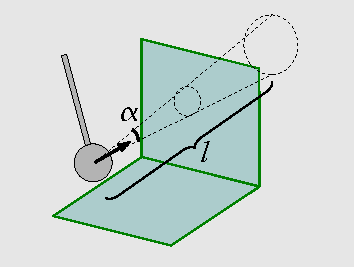
\includegraphics[width=3.2cm]{training}
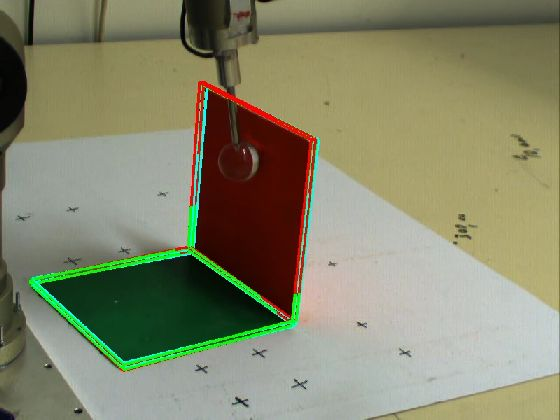
\includegraphics[width=3.2cm]{complex1}
}
\centerline{
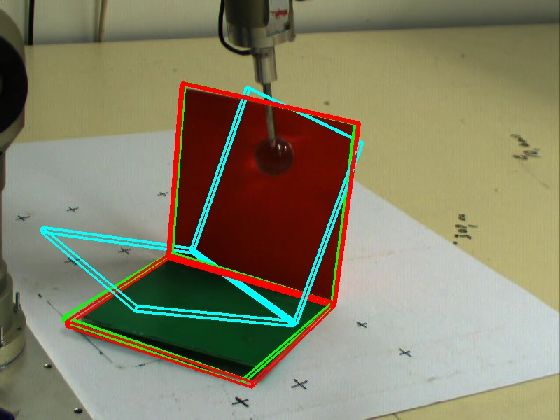
\includegraphics[width=3.2cm]{complex2}
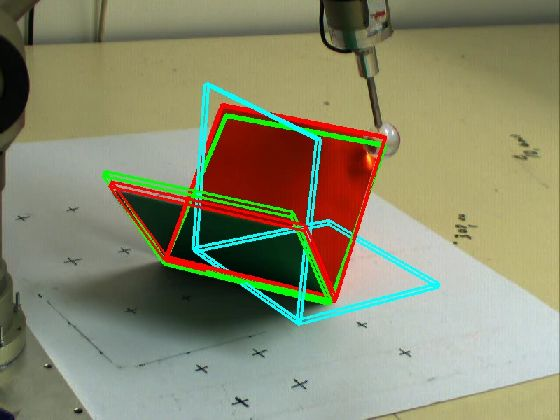
\includegraphics[width=3.2cm]{complex4}
}
\caption[Setup]{ In all experiments the robot finger pushes in a straight-line of length $l$=25$\pm$5 cm within a cone of angle $\alpha$=20 deg toward an object (top left). The start point is randomised so that each region on the vertical face is equally likely to be pushed. The red wire-frame shows the output of the visual tracker, the green wire-frame the object pose predicted by the KDEF learner, and the blue wire-frame the prediction of the PhysX simulator.}
\label{fig:Setup}
\end{figure}

Local frames for environment contacts in the -GAE variants were fixed
by hand to the edges of objects. In test cases with new objects the
frames were again fixed by hand.  An item for future work is to
perform this process automatically.  All methods required parameter tuning. Model selection was performed in experiment P1 to establish reasonable parameter values, which were then used in experiments P2 and P3.  It was not possible to perform fully systematic optimisations for LWPR, KDE and KDEF due to the size of the parameter spaces.  Rather, subsets of the parameter space were selected by inspection and then explored using grid search.  Models were evaluated on a separate hold-out set, of the same size as the test set. Model selection by full grid search was performed for the following parameters of the PhysX simulator: static friction, dynamic friction and the coefficient of restitution. PhysX has access to full mesh and contact information. In addition to model selection the three different parameterisations (Gauss-Euler (e), Gauss-Quaternion (q), Von-Mises-Fisher-Quat (v)) of rotations for the density estimation method were studied in experiment P1, and subsequently the best solution was used in experiments P2 and P3. For LWPR we used the Euler parameterisation throughout experiments P1, P2 and P3. For experiment P1 we performed 10-fold cross-validation. The sizes of the training and test sets are stated in the method for each experiment. For transfer learning experiments P2 and P3, disjoint training and test sets were used. For clarity a complete set of acronyms for the algorithm-information combinations is given in Table~\ref{tab:algs}. 
\begin{table}[b]
\begin{center}
\label{tab:algs}
\begin{tabular}{|l|l|l|l|}\hline
 & \multicolumn{3}{|c|}{Information} \\ \hline
Predictor & G & G+A & G+A+E \\ \hline
LWPR & LWPR-G& LWPR-GA & LWPR-GAE \\ \hline
KDE & KDE-G & KDE-GA & KDE-GAE \\ \hline
KDEF & KDEF-G & KDEF-GA & KDEF-GAE \\ \hline
PhysX & n/a & n/a & n/a \\ \hline
\end{tabular}
\caption{Algorithm-information variants.}
\end{center}
\end{table}
%%%%%%%%%%%%%%%%%%%%%%%%%%%%%%%%%%%%%%%%%%%%%%%%%%%%%%%%%%%%%%%%%%%%%%%
\subsection{Performance measure}\label{sec:Experiment.Performance}

In all experiments with real objects, predicted trajectories were evaluated against the visual tracked object pose. The tracker does not provide perfect ground-truth, yielding errors of $\pm$2mm. Prediction performance is evaluated as follows.

At any particular time step, $t$, a large number, $N$, of randomly chosen points $p_{n}^{1,t}$, where $n=1 \ldots N$, are rigidly attached to an object at the ground-truth pose, and the corresponding points $p_{n}^{2,t}$ to an object at the predicted pose. At time step $t$, an average error $E_t$ can now be defined as the mean of displacements between points on the object at the predicted pose and points on the object at the ground-truth pose:
\begin{equation}
E_t = \frac{1}{N} \mathop{\sum}_{n=1 \ldots N}|p_{n}^{2,t}-p_{n}^{1,t}|
\label{eq:defn_Rt}
\end{equation}
Note that for each push action, we predict approximately 150
consecutive steps into the future, with no recursive filtering or
corrector steps, hence it is expected that errors will grow with range
from the initial object pose. We therefore find it more meaningful to
normalise all errors with respect to an ``average range'', $R_t$, of
the object from its starting position, defined as:
\begin{equation}
R_t = \frac{1}{N} \mathop{\sum}_{n=1 \ldots N}|p_{n}^{1,t}-p_{n}^{1,0}|
\label{eq:defn_Et}
\end{equation}
For a test data set, consisting of $K$ robotic pushes, each of which breaks down into many consecutive predictions over $T$ time steps, we can now define average error and normalised average error. Note that the normalised error measure necessarily has no units.
\begin{align}
E_{av} &= \frac{1}{K} \mathop{\sum}_{k=1}^{K} \frac{1}{T} \mathop{\sum}_{t=1}^{T} E_t,
&E_{av}^{norm} &= \frac{1}{K} \mathop{\sum}_{k=1}^{K} \frac{1}{T} \mathop{\sum}_{t=1}^{T} \frac{E_t}{R_t}
\label{eq:Error1}
\end{align}


\begin{figure*}[t]
\centerline{
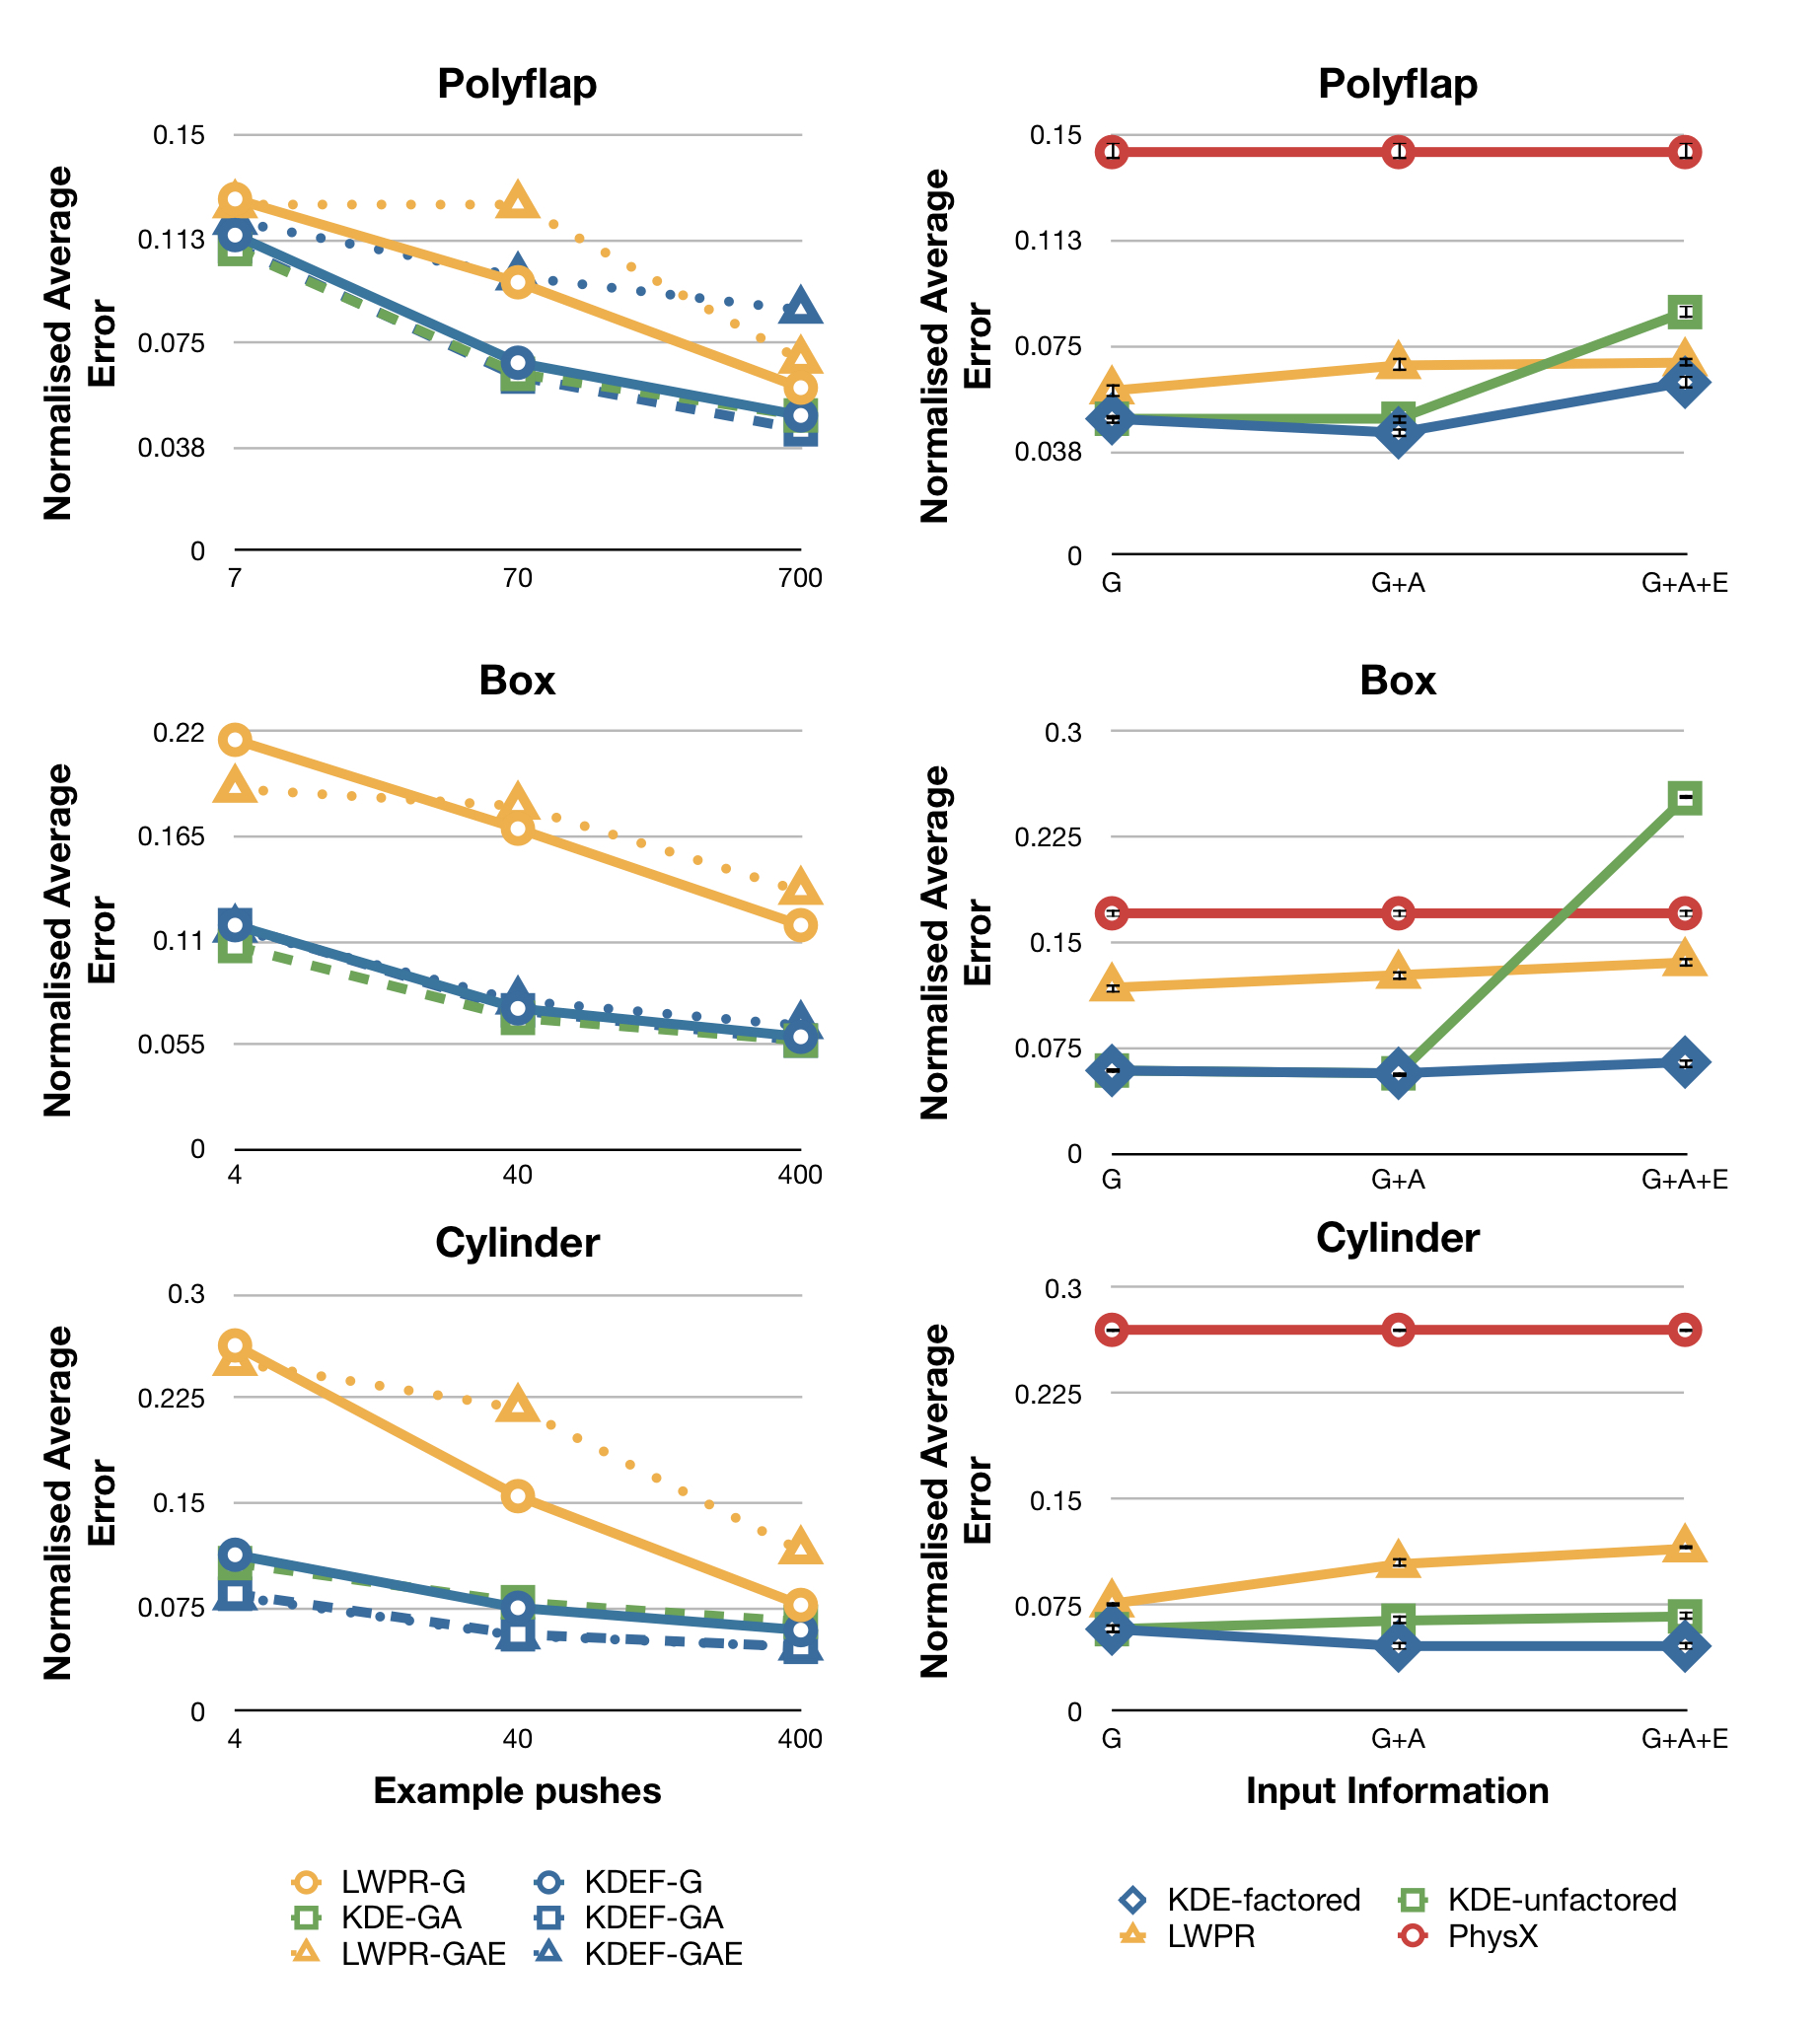
\includegraphics[width=0.8\textwidth]{graphs_jw/P1-graphs}
%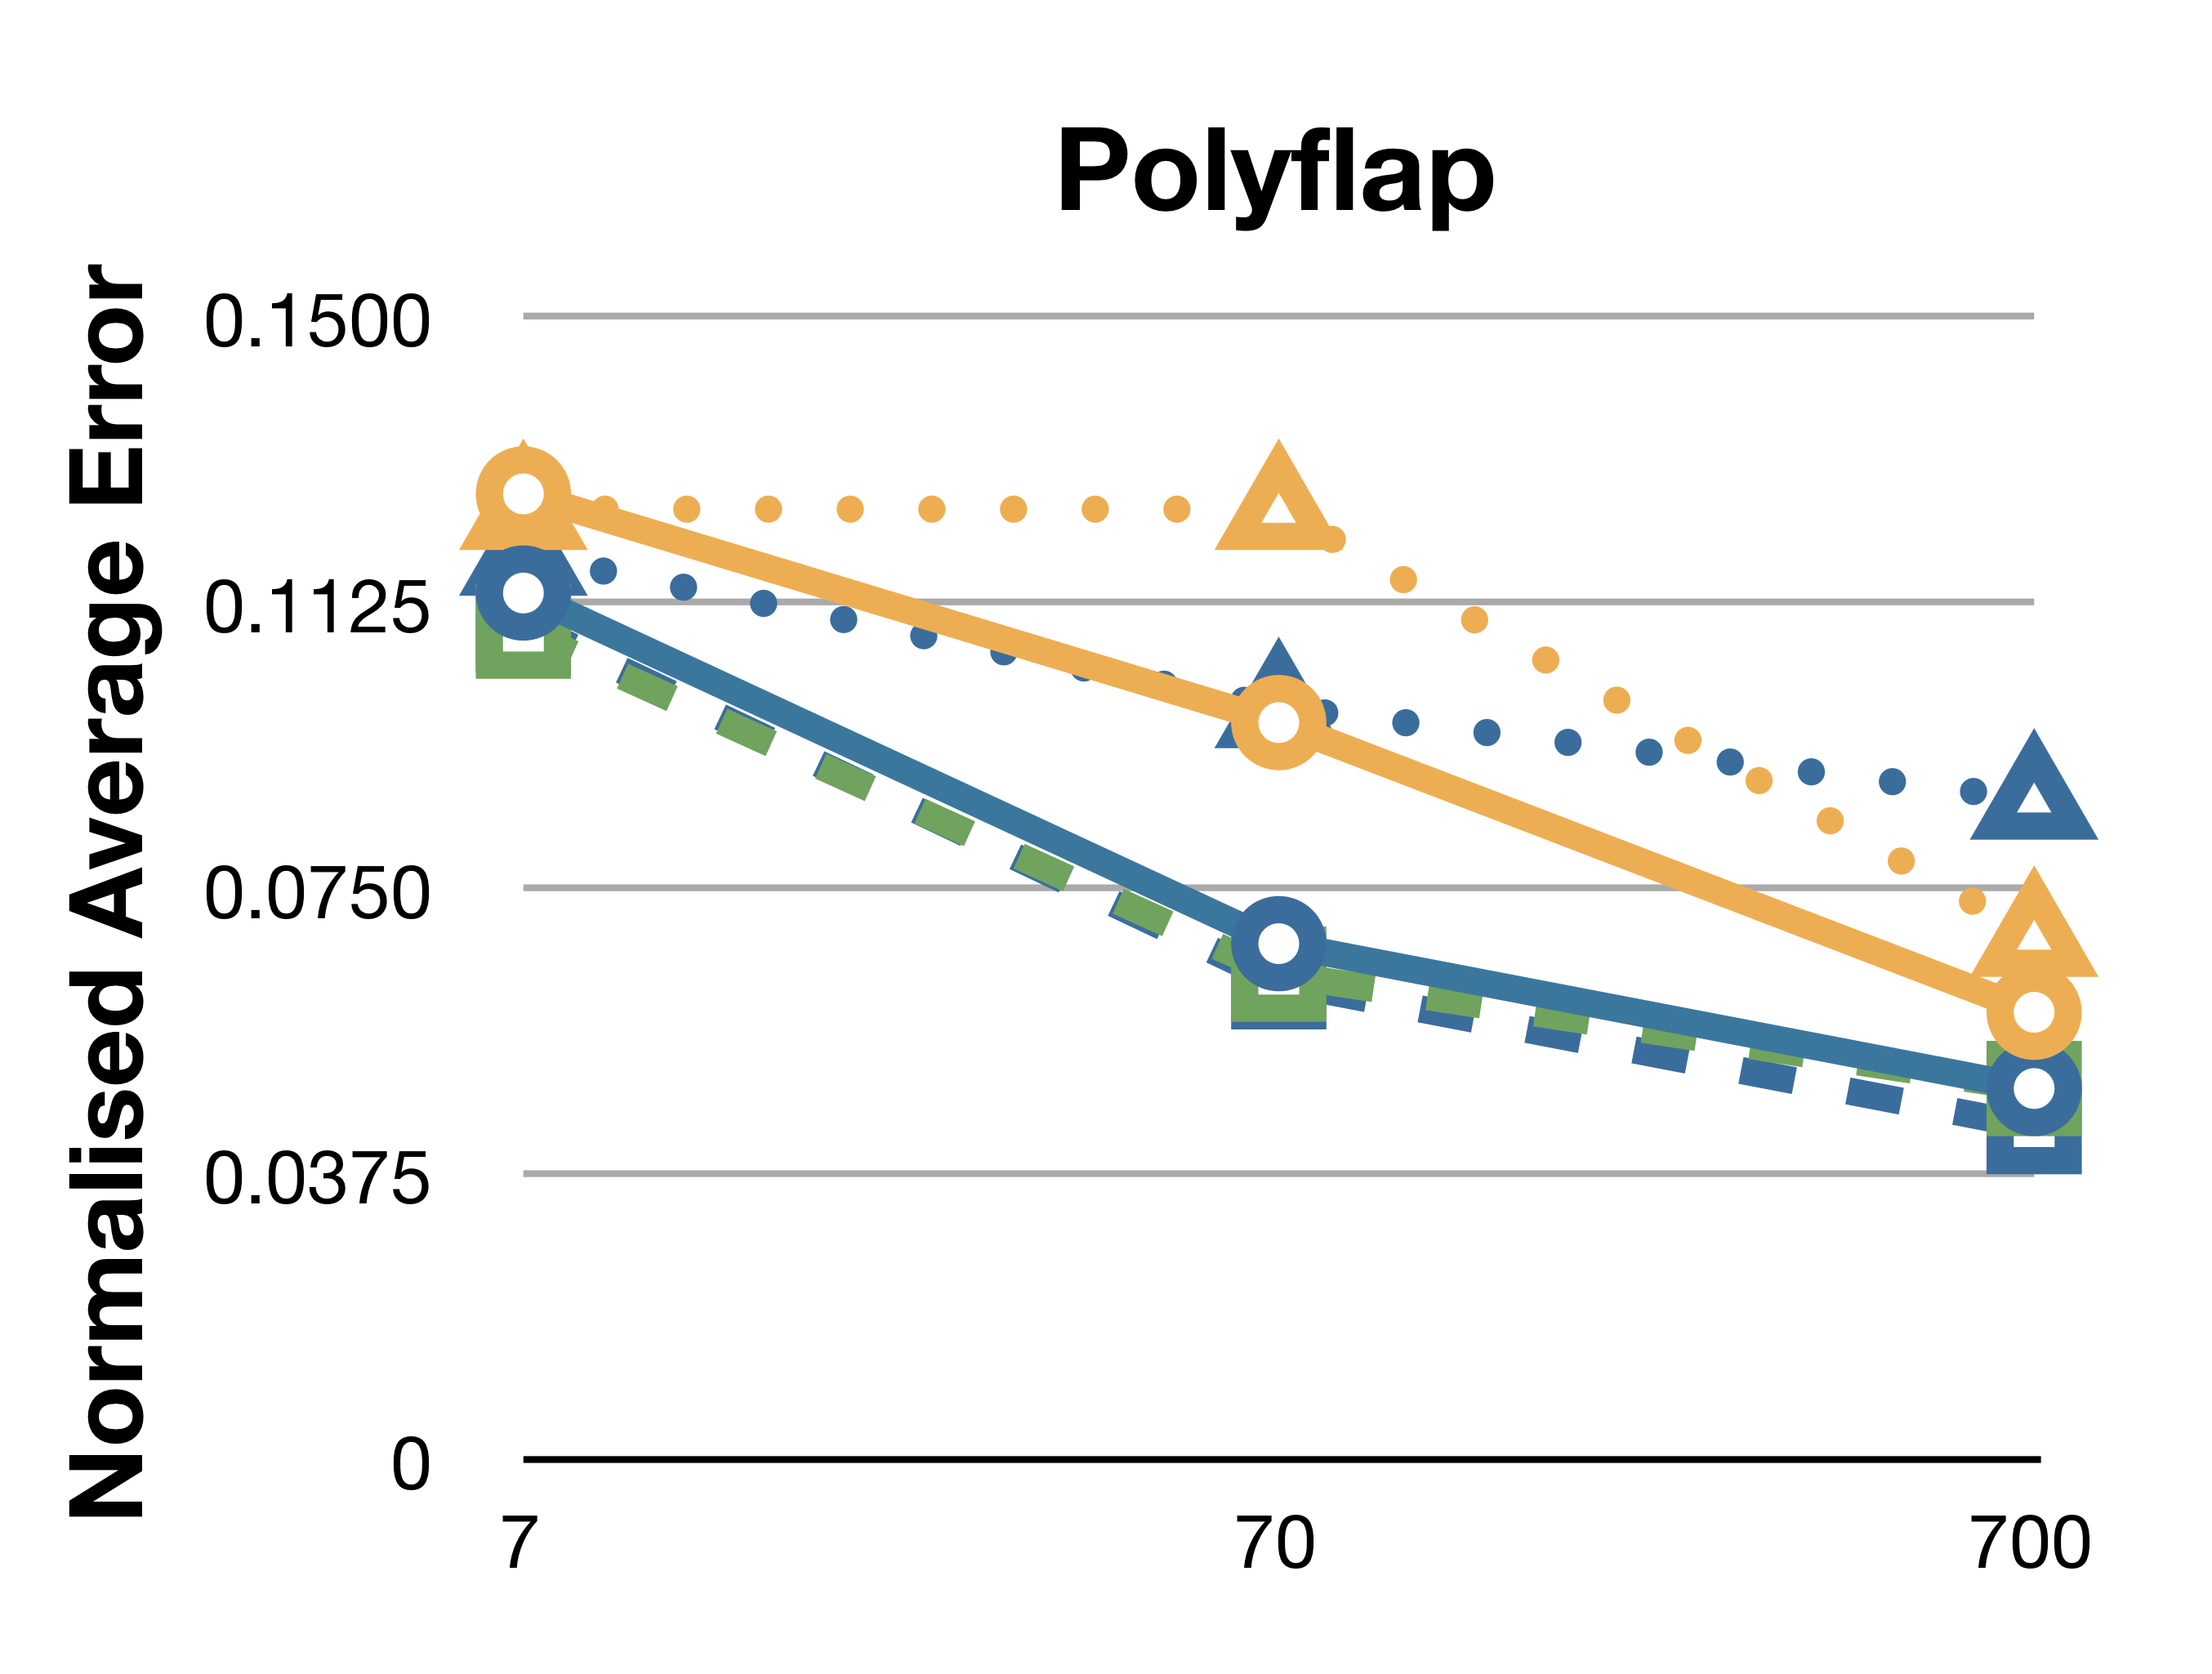
\includegraphics[width=0.45\columnwidth]{graphs_jw/L1av_graph}
%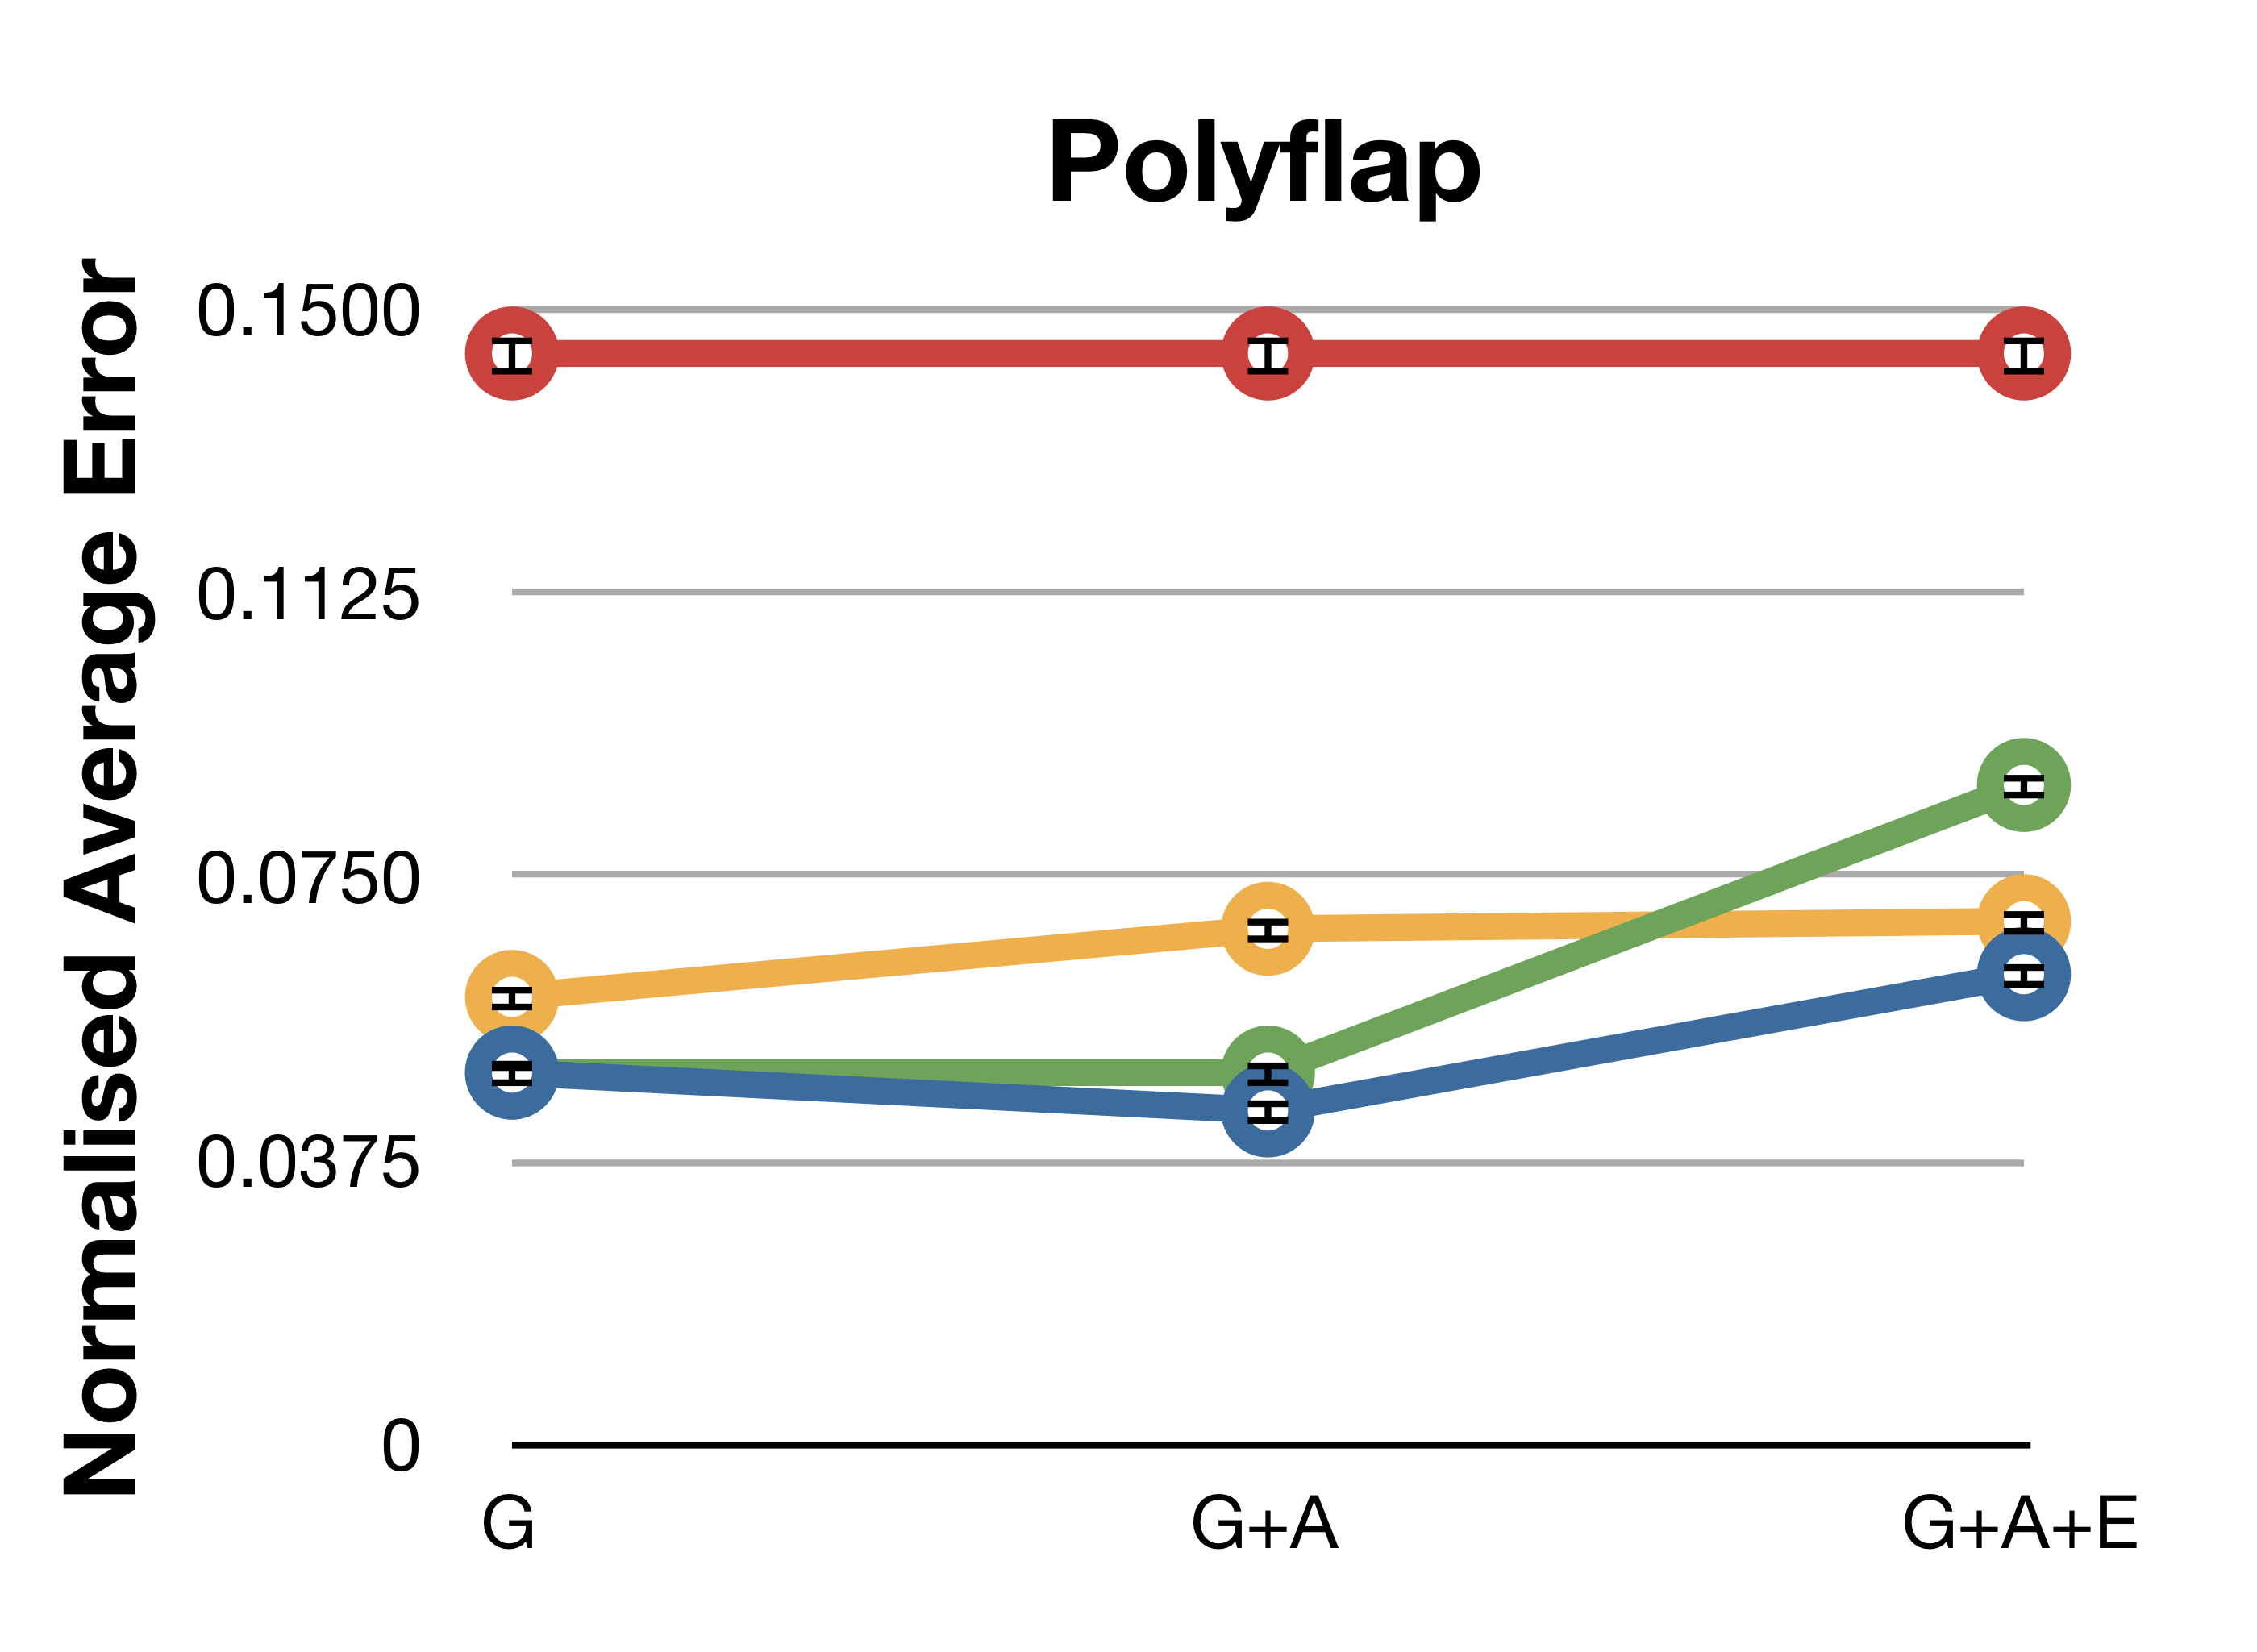
\includegraphics[width=0.45\columnwidth]{graphs_jw/L1av_graph_polyflap}
%}
%\centerline{
%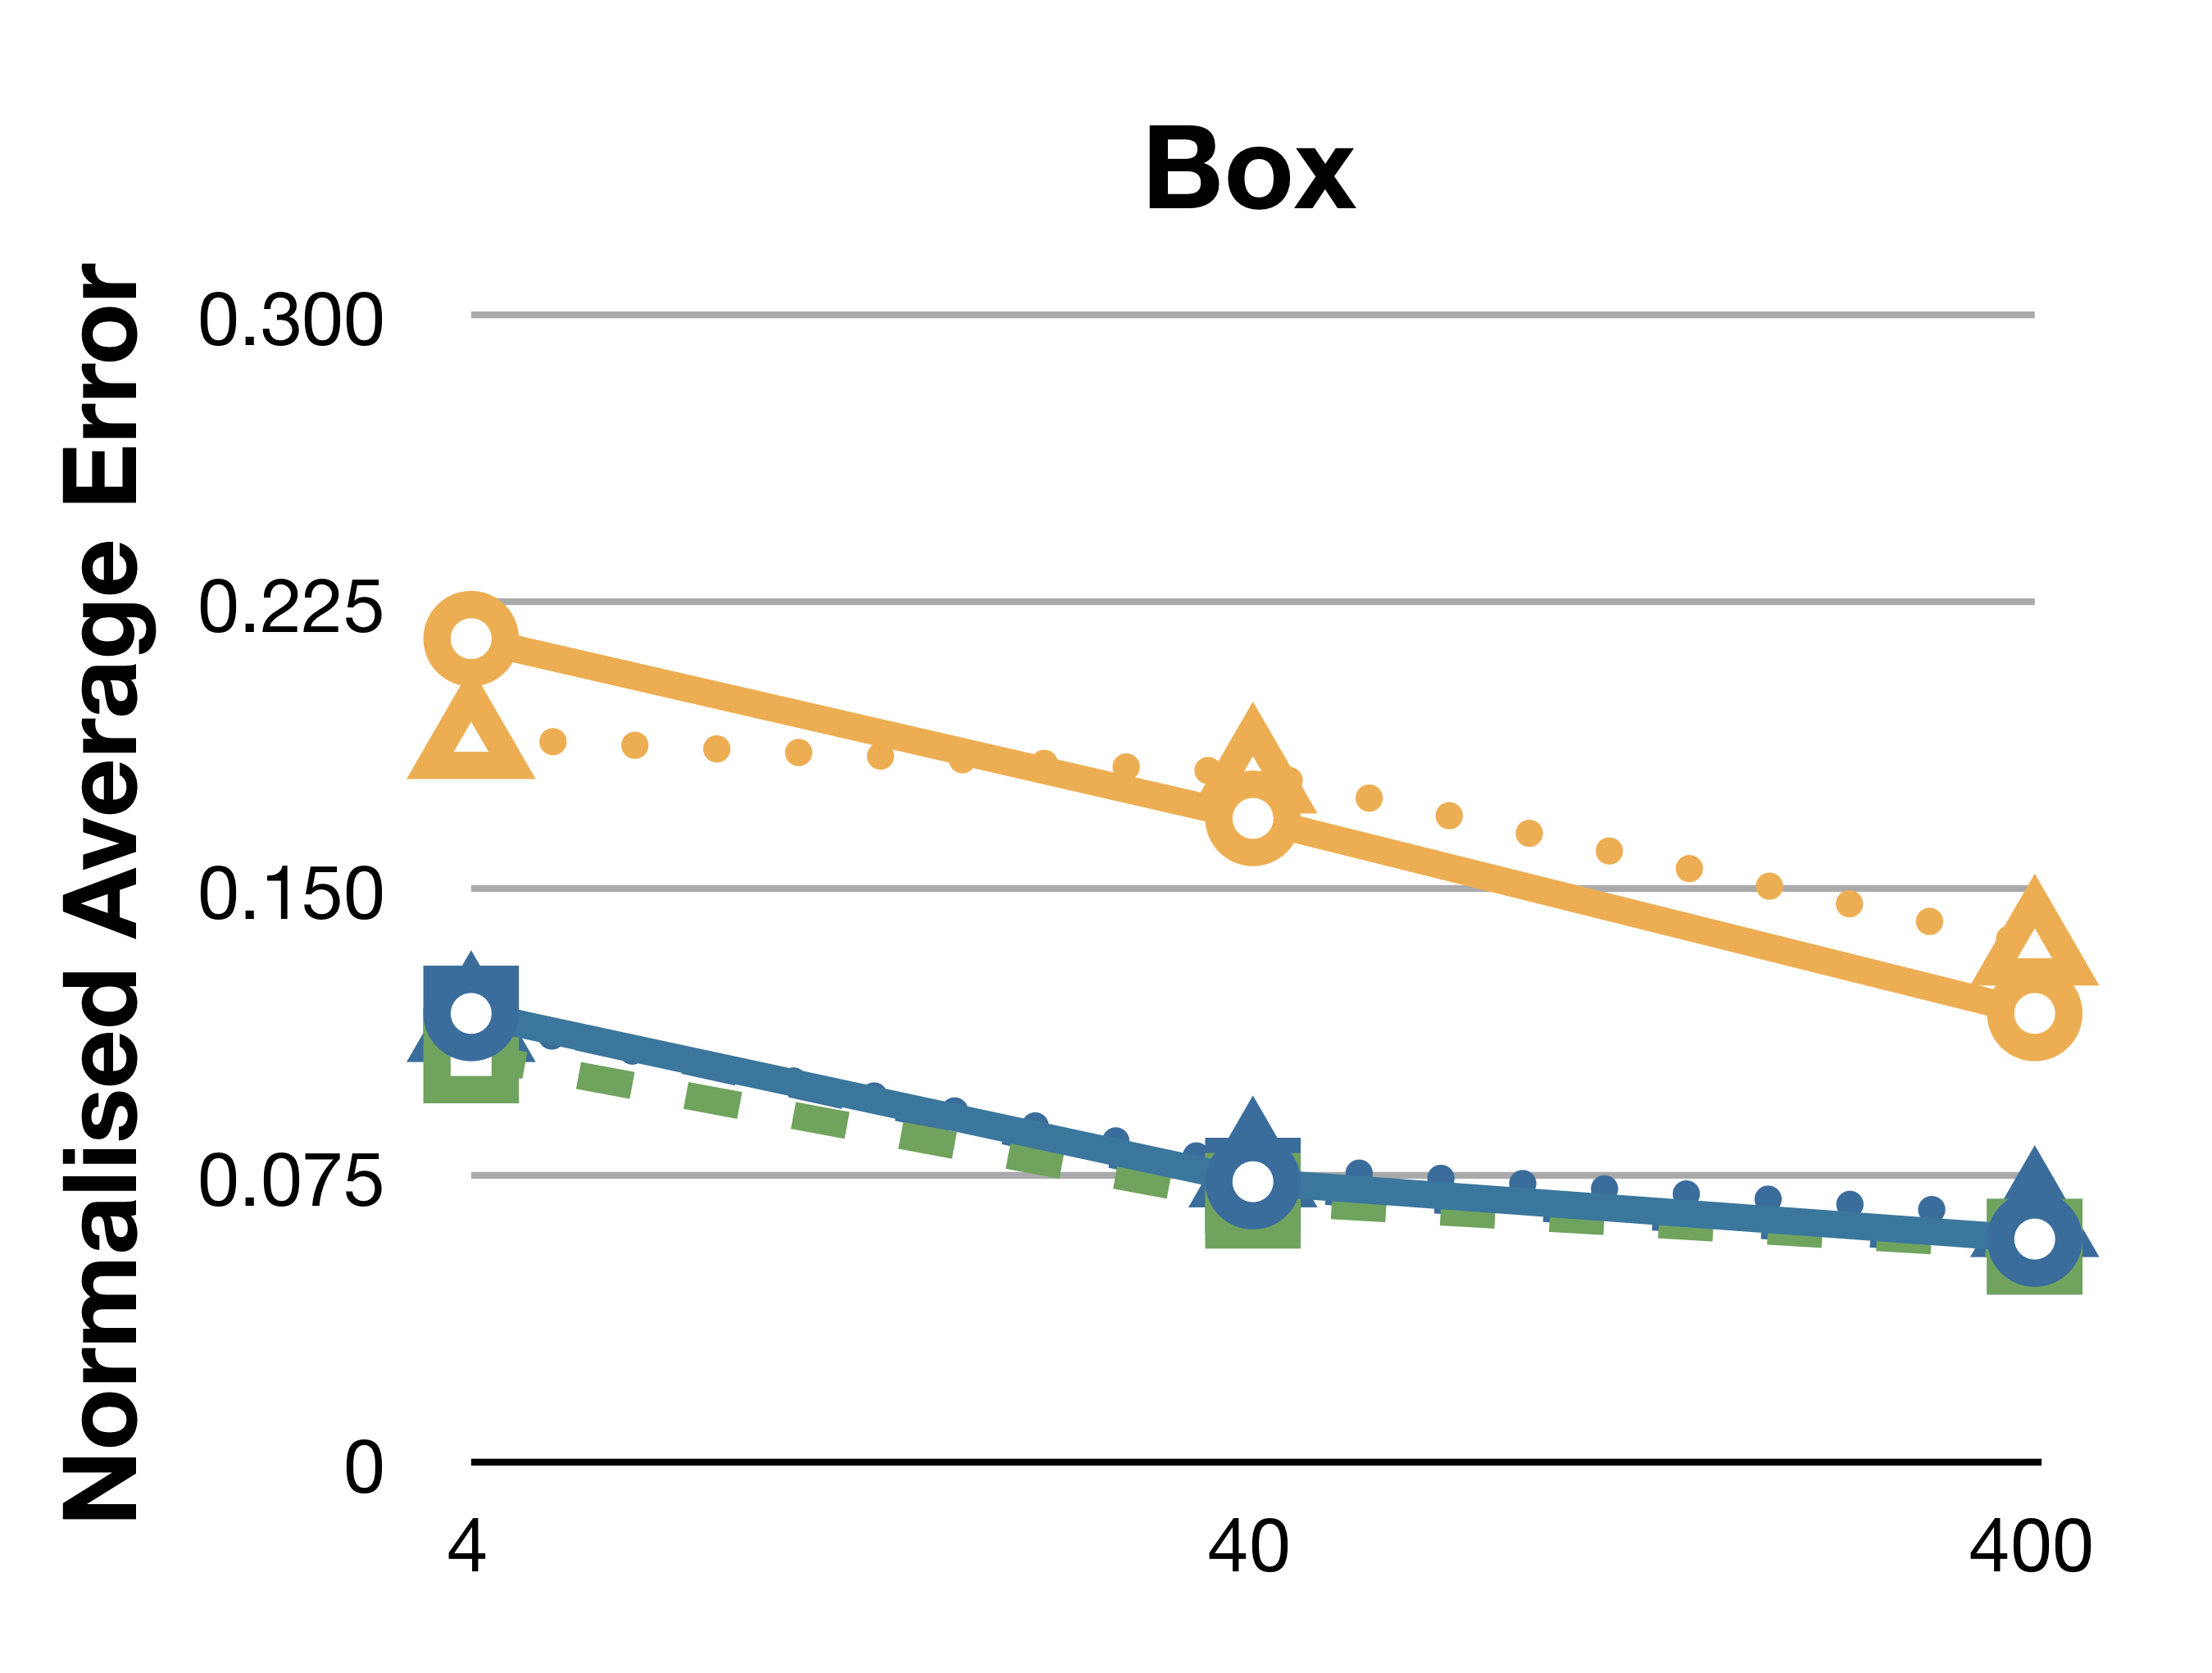
\includegraphics[width=0.45\columnwidth]{graphs_jw/L2av_graph}
%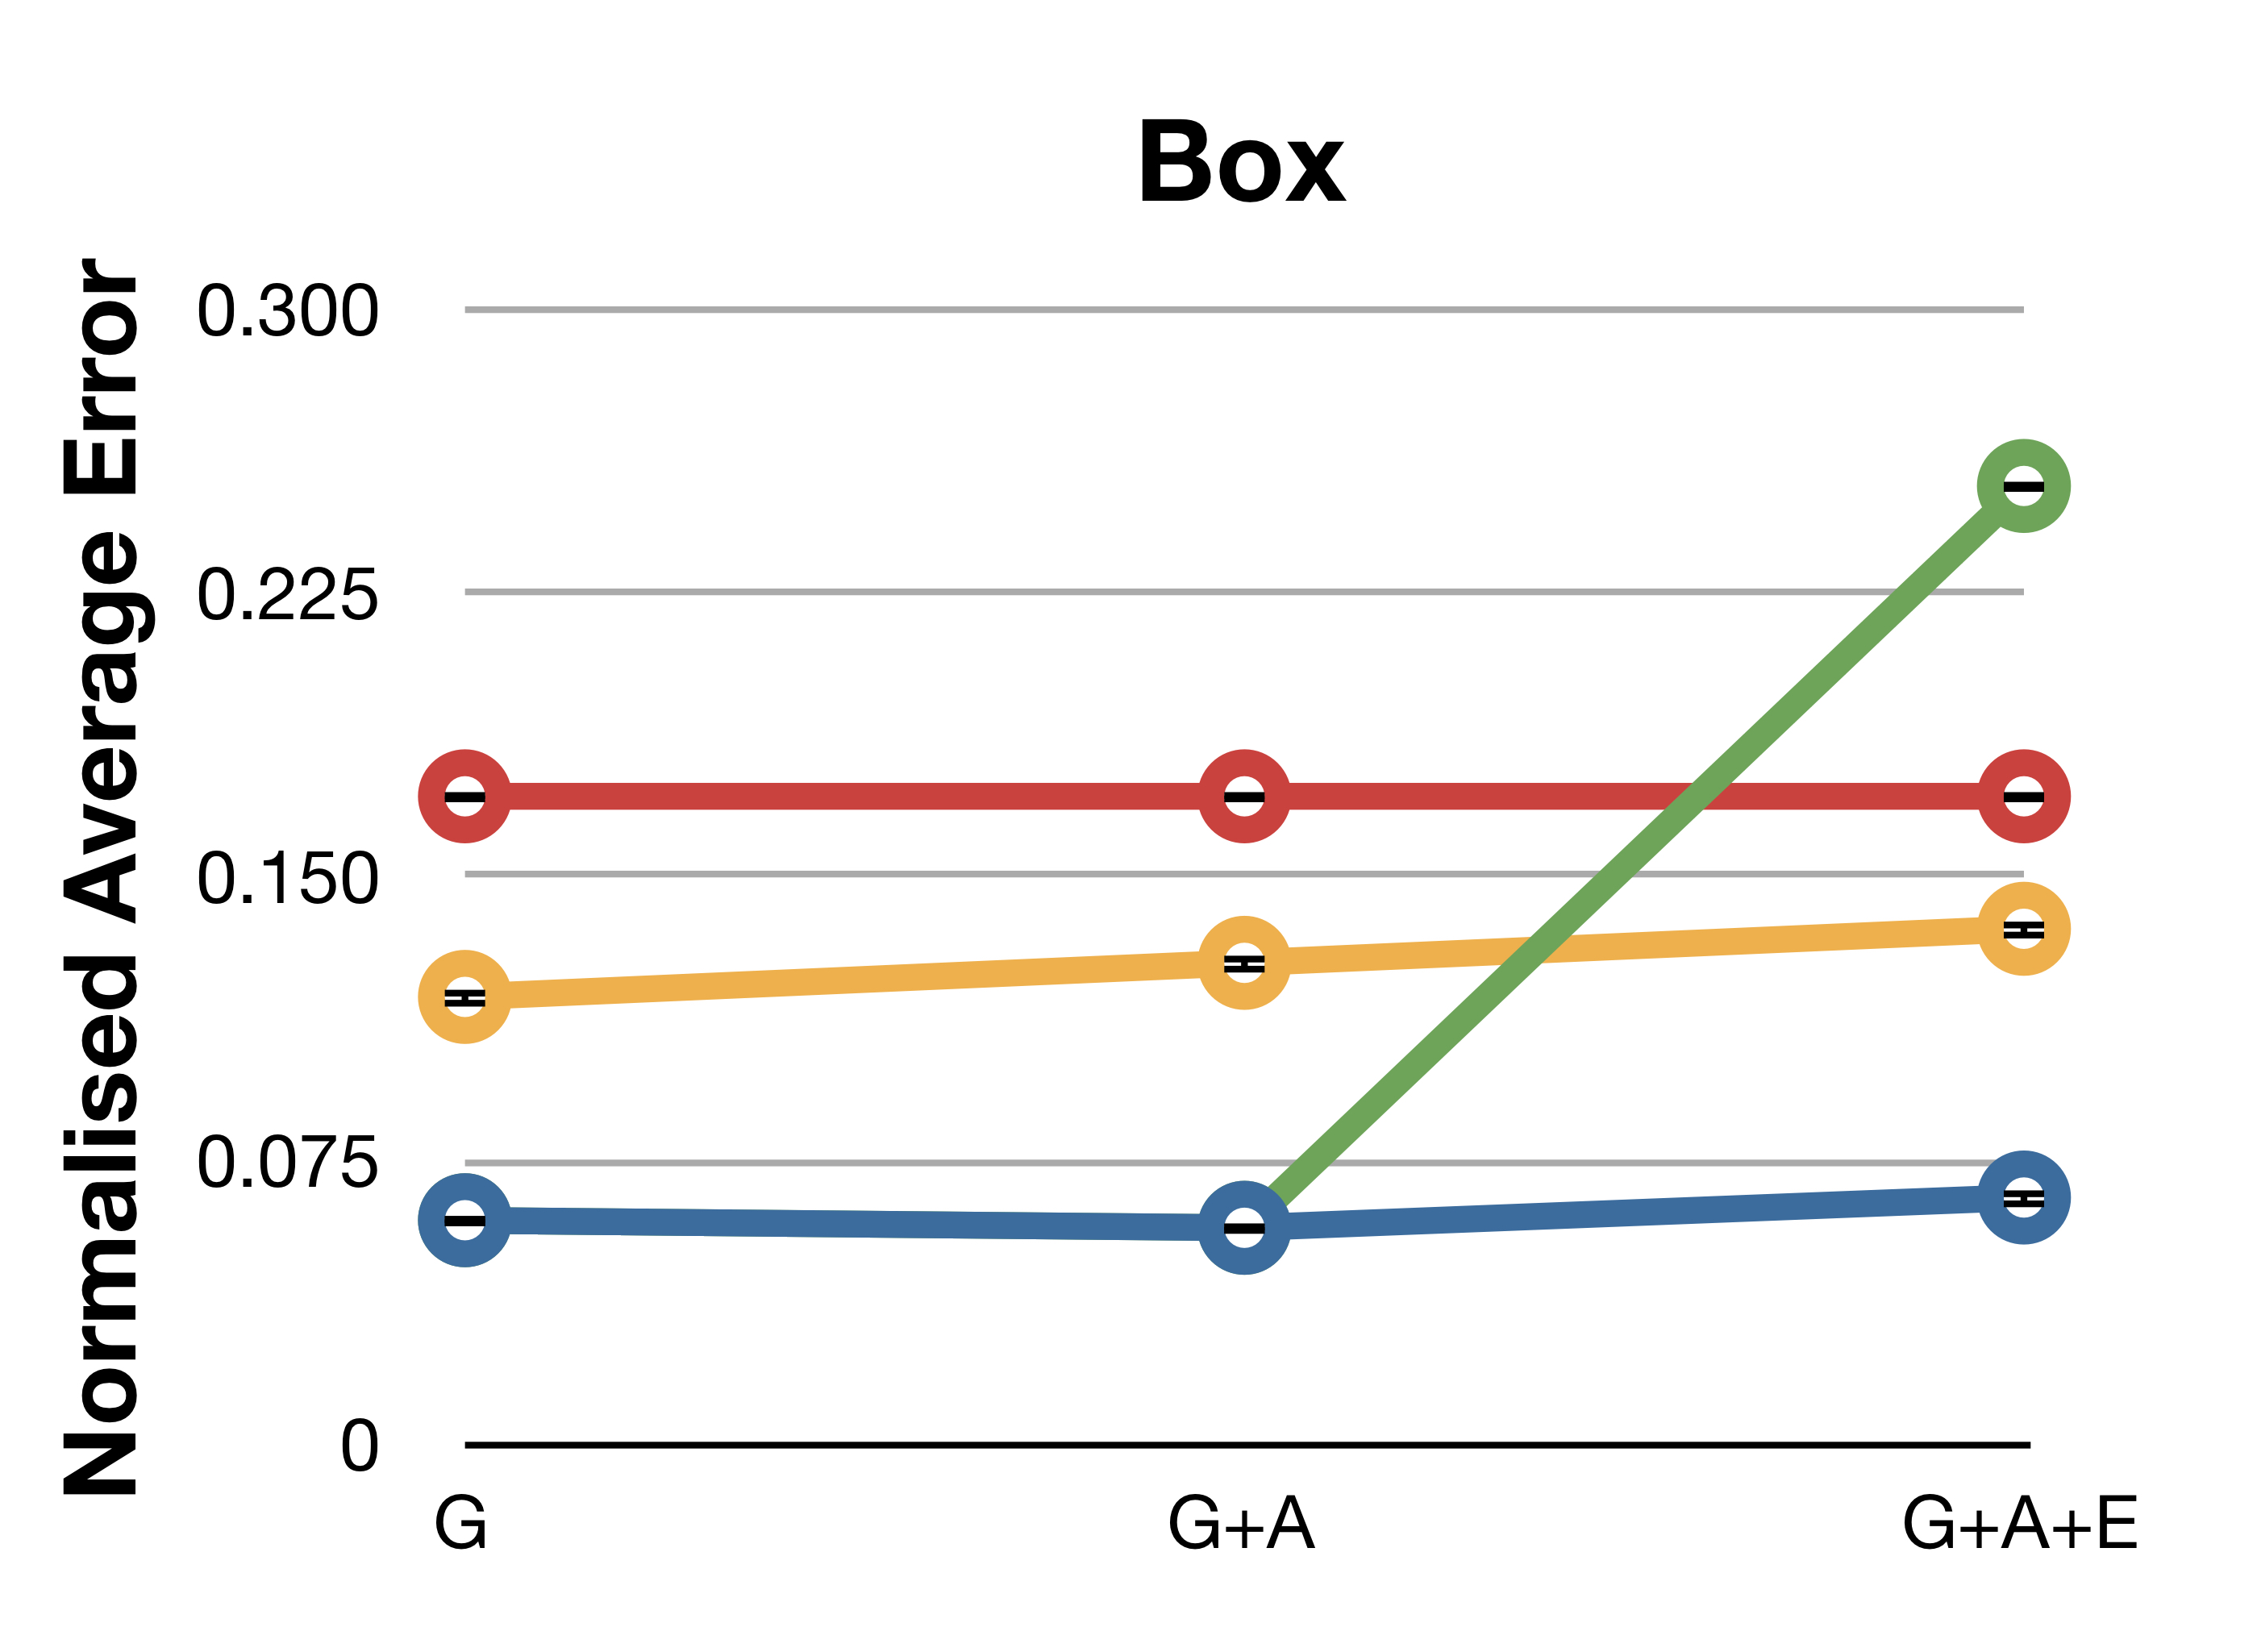
\includegraphics[width=0.45\columnwidth]{graphs_jw/L1av_graph_box}
%}
%\centerline{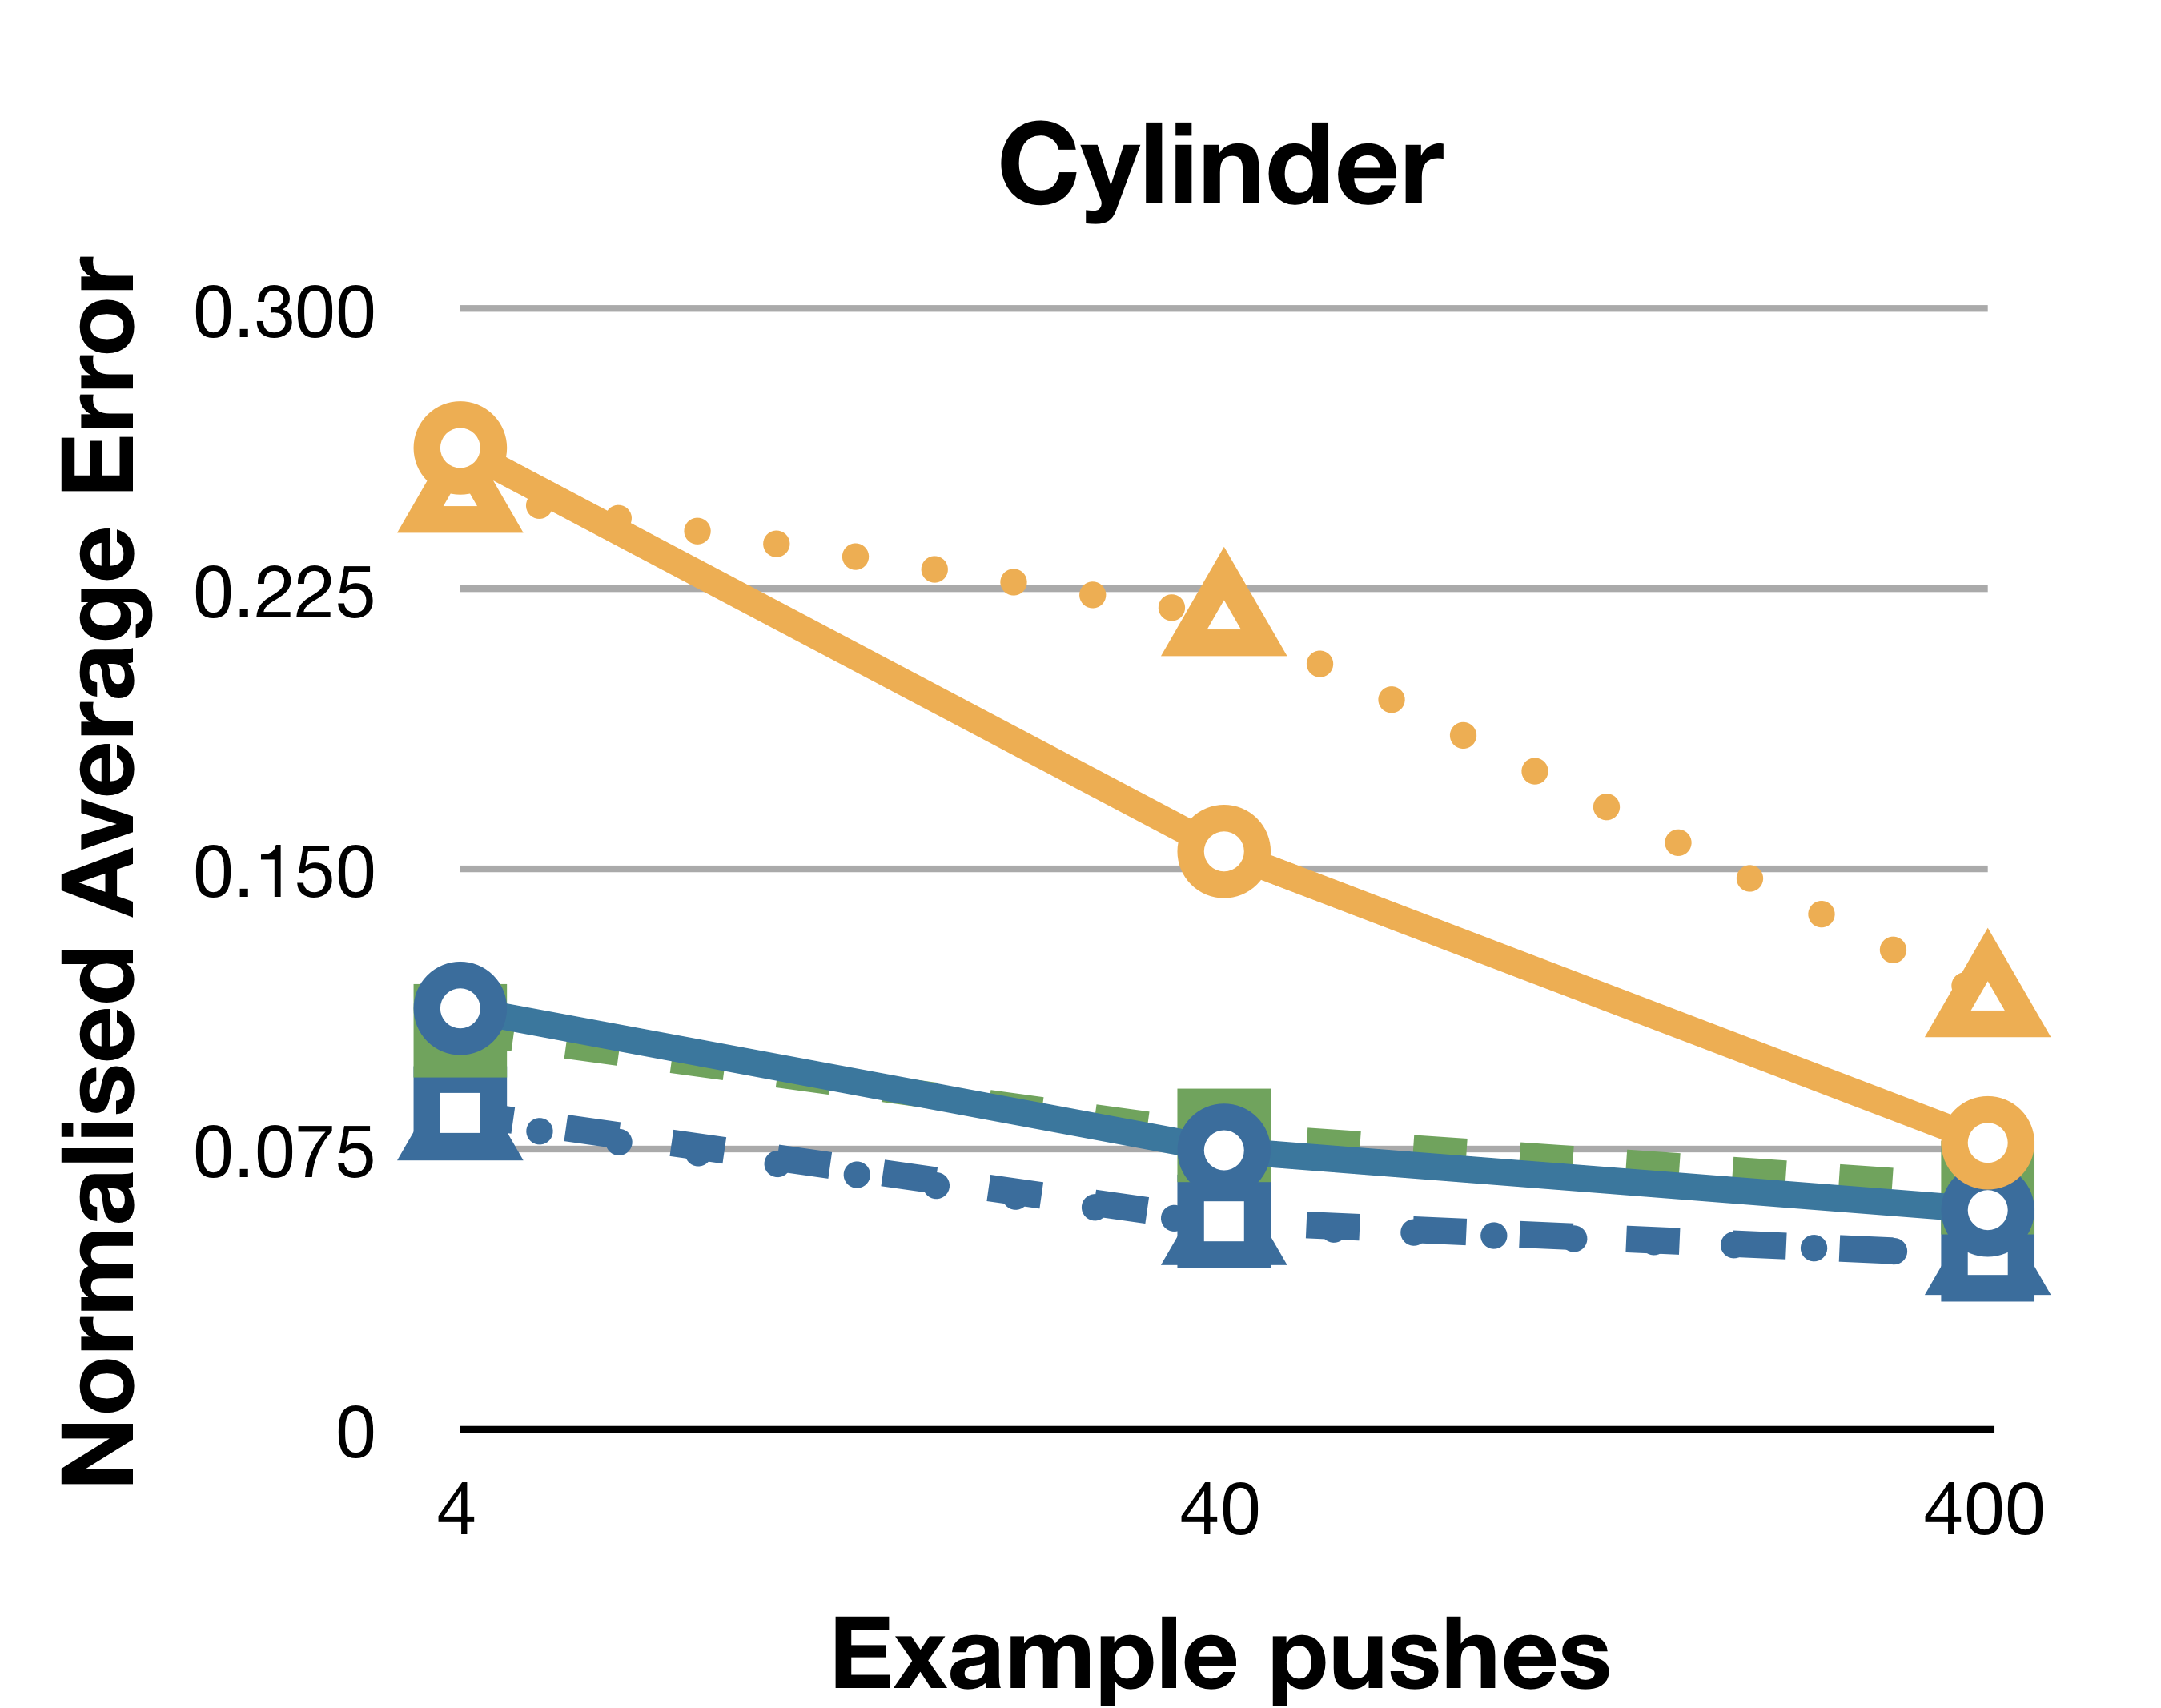
\includegraphics[width=0.45\columnwidth]{graphs_jw/L3av_graph}
%                 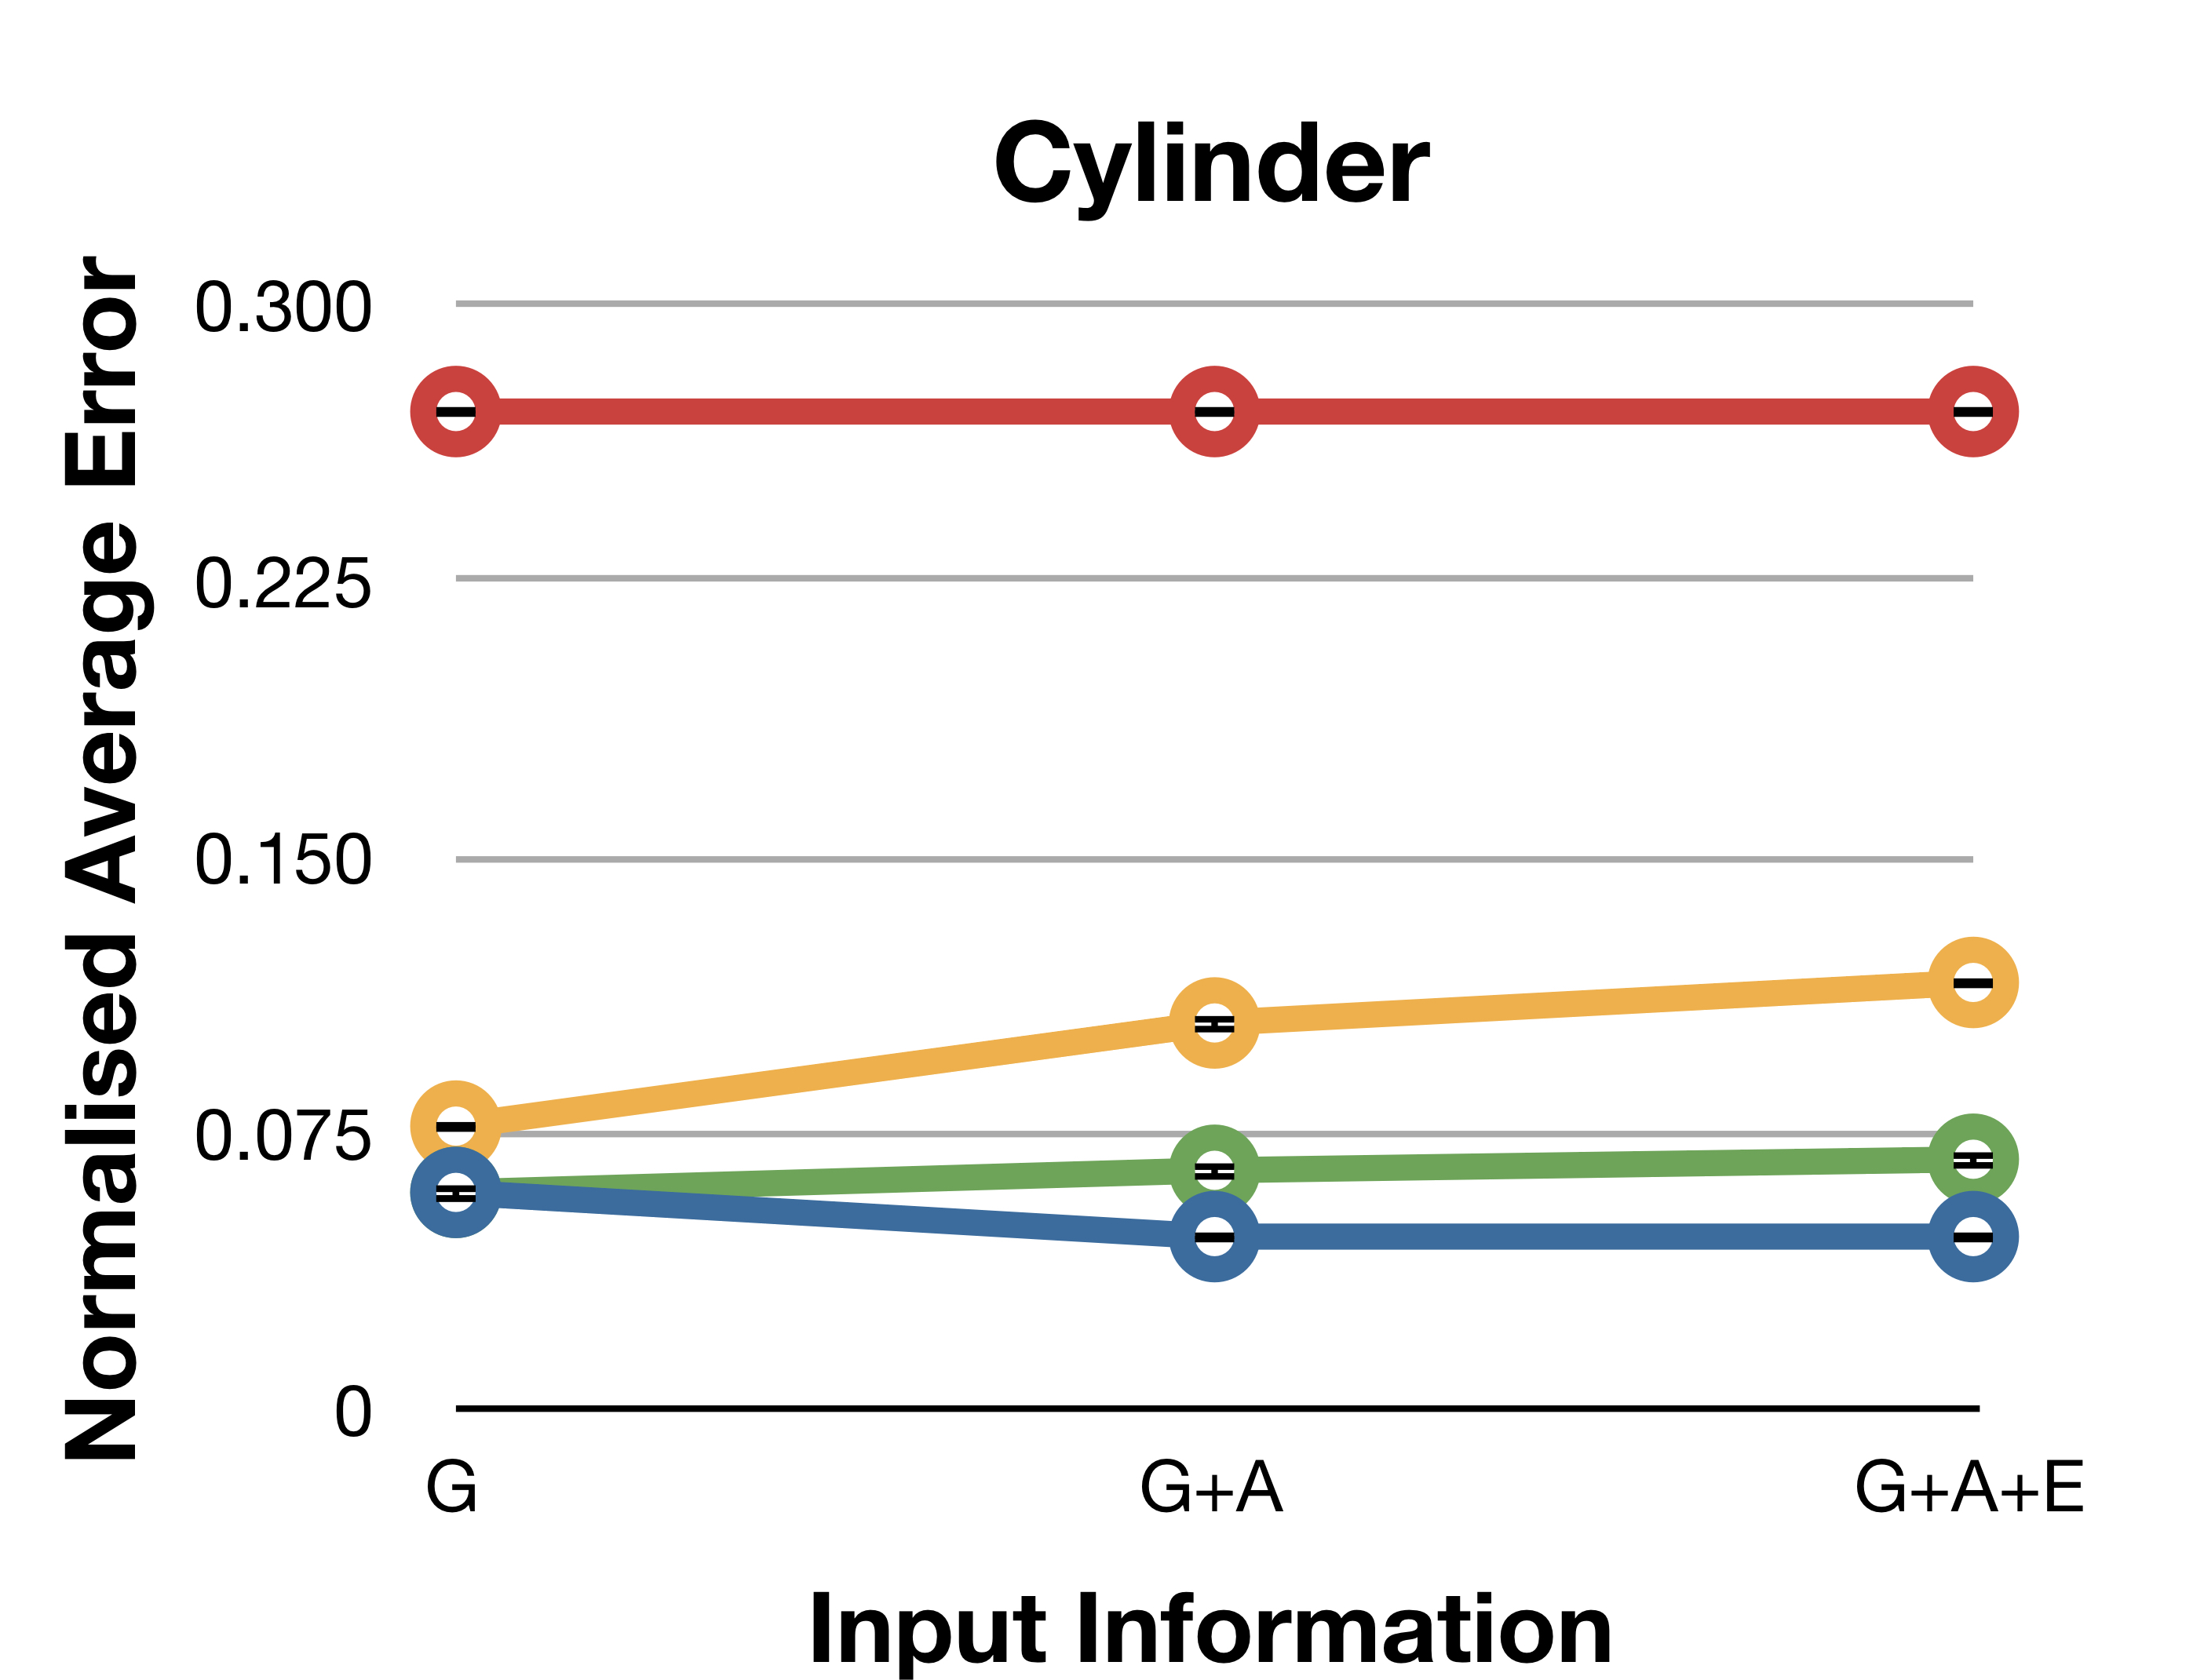
\includegraphics[width=0.45\columnwidth]{graphs_jw/L1av_graph_cylinder}
%}
%\centerline{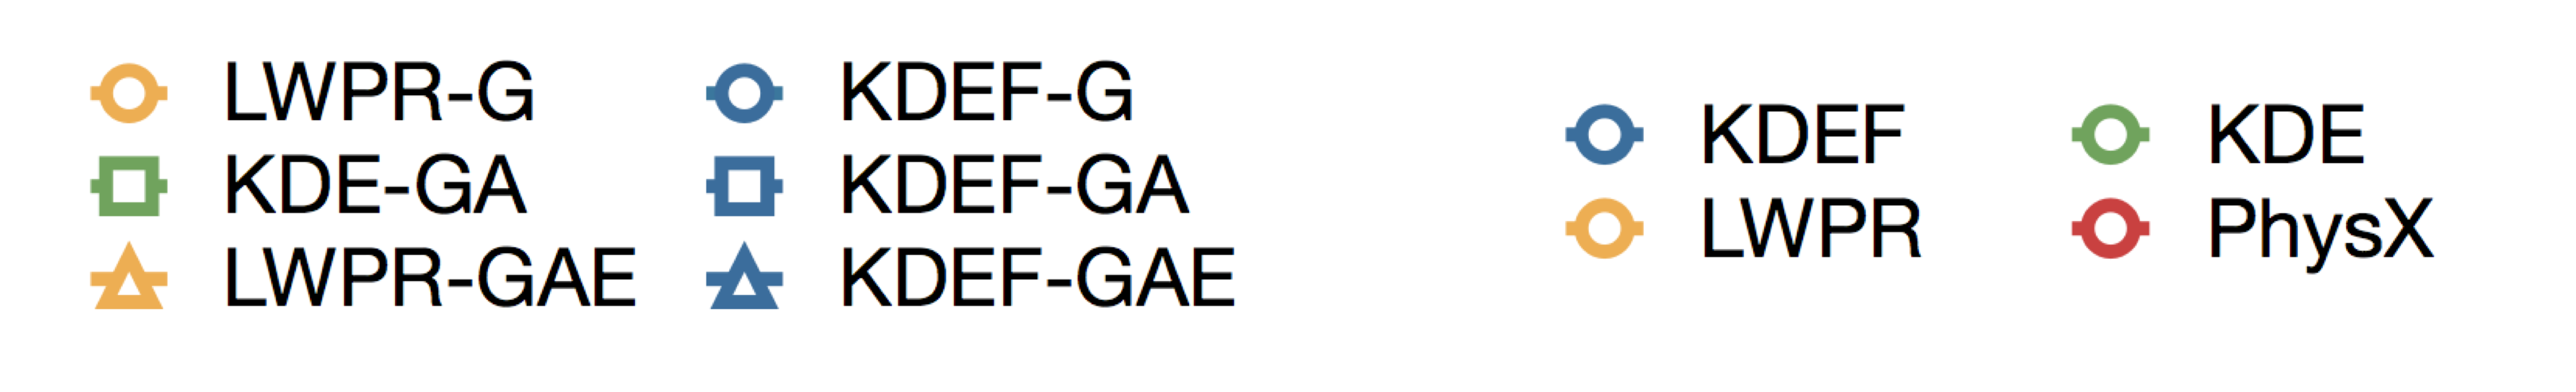
\includegraphics[width=\linewidth]{graphs_jw/L1_convergence_graph_key}
}
\vspace{-1mm}
\caption{Experiment P1: Convergence of a selection of learning
  algorithm-information combinations (left column). Change in normalised average prediction errors with varying input information (right column). G - global information; A - agent-object information; E - object-environment information.}
\label{fig:Lgraphs}
\end{figure*}


\section{Results}\label{sec:Results}

\subsection{Experiment P1: Action Interpolation}\label{sec:Results.Learning}

In Experiment P1 the robot applied a set of random pushes to a
polyflap, a box and a cylinder respectively. All the algorithm
variants in Table~\ref{tab:algs} were trained and tested. Model
selection was performed for all algorithm-information combinations including PhysX. Ten fold cross-validation was performed for all algorithms. The density estimation techniques were studied with all three parameterisations of rotation. Training (and testing) sets were 200 (25) pushes (cylinder), 400 (50) pushes (box) and 700 (90) pushes (polyflap). Figure~\ref{fig:Lgraphs} (left column) shows convergence of the best learning algorithms. Figure~\ref{fig:Lgraphs} (right column) shows how performance varies with input information for the best parameterisations of all the algorithms. Table~\ref{tab:PerformanceTableL1av} shows the results of model selection on the different parameterisations for KDE. Image sequences of predicted vs actual trajectories are shown in (Figure~\ref{fig:ExperimentL2}).

\begin{table*}[t]
\begin{center}

\label{tab:PerformanceTableL1av}
\begin{tabular}{|l|l|l|l|l|}
\cline{1-4}
Predictor & Polyflap & Box & Cylinder \\
\cline{1-4}
KDEF-Ge & 0.055$\pm$0.002 & 0.061$\pm$0.003 & 0.063$\pm$0.003\\
KDEF-Gq  & \textbf{0.049}$\pm$0.002 & \textbf{0.059}$\pm$0.002 & \textbf{0.059}$\pm$0.003\\
KDEF-Gv   & 0.057$\pm$0.002 & 0.066$\pm$0.003 & 0.071$\pm$0.003\\
LWPR-Ge &  0.059$\pm$0.002 & 0.118$\pm$0.003 & 0.077$\pm$0.003\\
\cline{1-4}
KDEF-GAe & 0.054$\pm$0.002 & 0.060$\pm$0.003 & 0.052$\pm$0.002\\
KDEF-GAq & \textbf{0.044}$\pm$0.002 & \textbf{0.057}$\pm$0.002 & \textbf{0.047}$\pm$0.002\\
KDEF-GAv  & 0.064$\pm$0.002 & 0.097$\pm$0.002  & 0.109$\pm$0.003 \\
LWPR-GAe & 0.068$\pm$0.002 & 0.127$\pm$0.003 & 0.105$\pm$0.002 \\
\cline{1-4}
KDEF-GAEe & 0.083$\pm$0.003 & 0.065$\pm$0.003 & 0.050$\pm$0.002 \\
KDEF-GAEq & \textbf{0.062}$\pm$0.002 & \textbf{0.065}$\pm$0.003 & \textbf{0.047}$\pm$0.002\\
KDEF-GAEv & 0.081$\pm$0.002 & 0.086$\pm$0.002 & 0.065$\pm$0.002\\
LWPR-GAEe & 0.069$\pm$0.002 & 0.136$\pm$0.003 & 0.116$\pm$0.003\\
\cline{1-4}
KDE-GAe & 0.053$\pm$0.002 & 0.057$\pm$0.002 & 0.068$\pm$0.003 \\
KDE-GAq  & \textbf{0.049}$\pm$0.002 & \textbf{0.057}$\pm$0.002 & \textbf{0.065}$\pm$0.003\\
KDE-GAv   & 0.062$\pm$0.002 & 0.058$\pm$0.002 & 0.092$\pm$0.004\\
\cline{1-4}
KDE-GAEe & 0.090$\pm$0.002 & 0.161$\pm$0.003 & 0.071$\pm$0.003\\
KDE-GAEq  & \textbf{0.087}$\pm$0.002 & 0.253$\pm$0.002 & \textbf{0.068}$\pm$0.003\\
KDE-GAEv   & \textbf{0.087}$\pm$0.002 & \textbf{0.127}$\pm$0.003 & 0.091$\pm$0.004\\
\cline{1-4}
PhysX & 0.144$\pm$0.003 &  0.171$\pm$0.003 & 0.271$\pm$0.001\\
\cline{1-4}
\end{tabular}
\caption[Performance Table]{Experiment P1: Forward push on a
  polyflap/box/cylinder, trained on real data. Shown is the dimensionless measure normalised average error  ${E_{av}^{norm}} \pm$ standard error. The parameterisations are denoted by e (Euler), q (Gauss Quaternion) and v (Von-Mises Fisher) respectively.
}
\end{center}
\end{table*}

\newlength{\imgAXwid}
\setlength{\imgAXwid}{2.07cm}

\begin{figure*}[htbp]
\centerline{
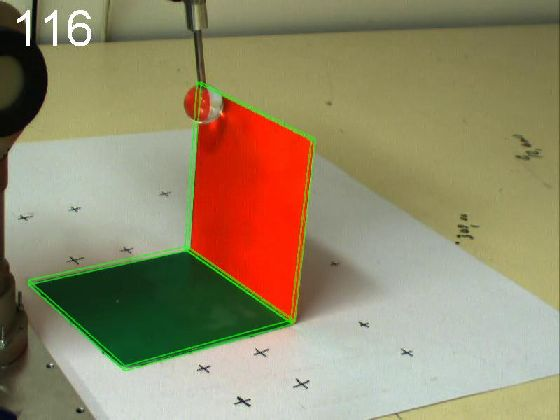
\includegraphics[width=\imgAXwid]{images/A1_2exp_667_1}
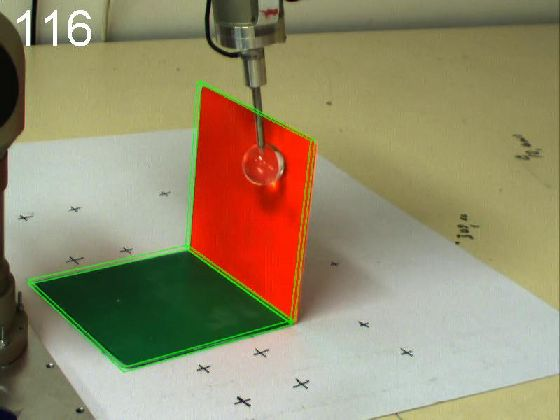
\includegraphics[width=\imgAXwid]{images/A1_2exp_876_1}
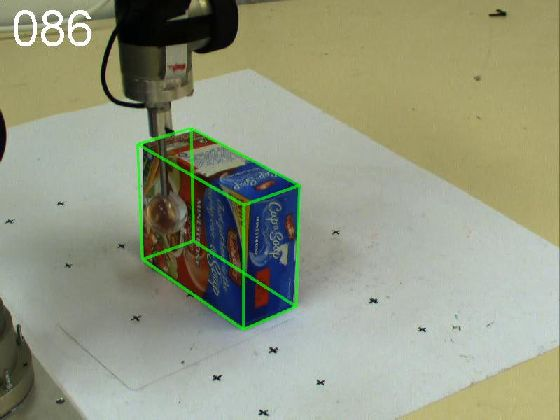
\includegraphics[width=\imgAXwid]{images/A2_2exp_399_1}
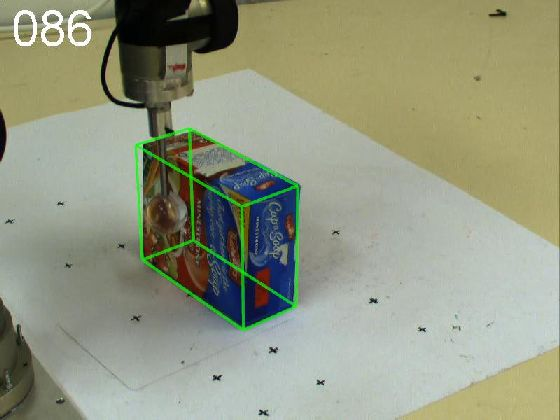
\includegraphics[width=\imgAXwid]{images/A2_LWPR1_399_1}
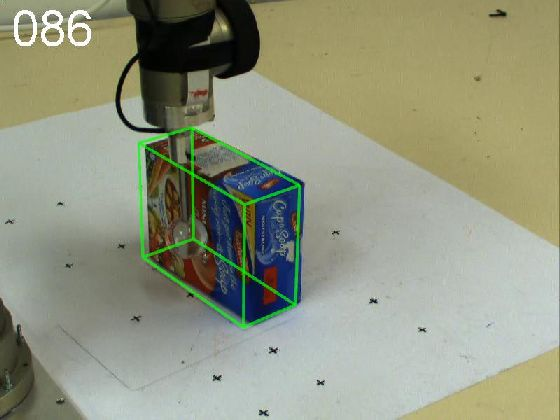
\includegraphics[width=\imgAXwid]{images/A2_2exp_87_1}
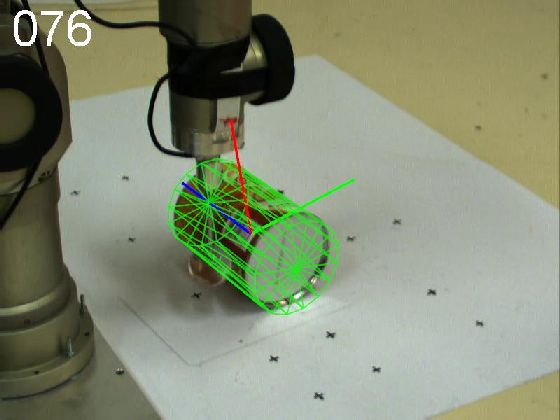
\includegraphics[width=\imgAXwid]{images/A3_2exp_39_1}
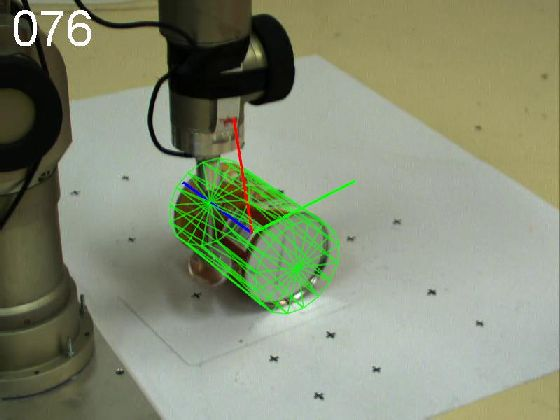
\includegraphics[width=\imgAXwid]{images/A3_LWPR1_39_1}
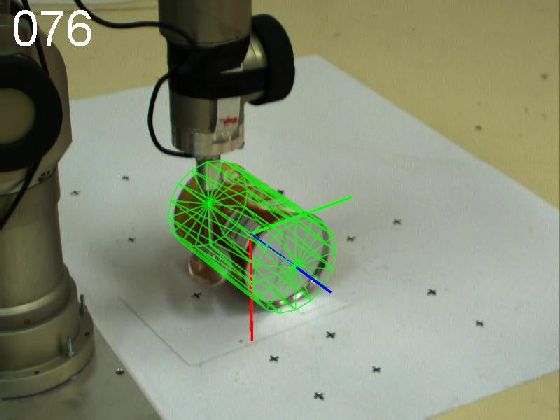
\includegraphics[width=\imgAXwid]{images/A3_physx_39_1}
}
\centerline{
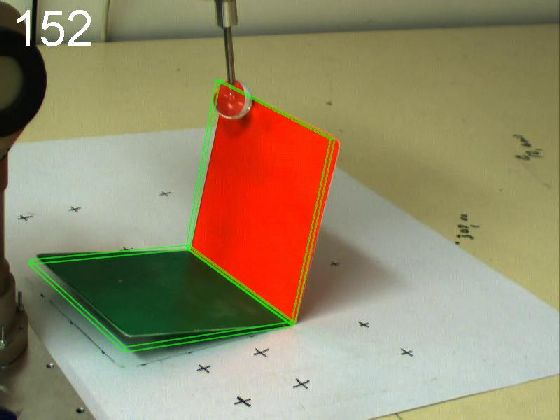
\includegraphics[width=\imgAXwid]{images/A1_2exp_667_2}
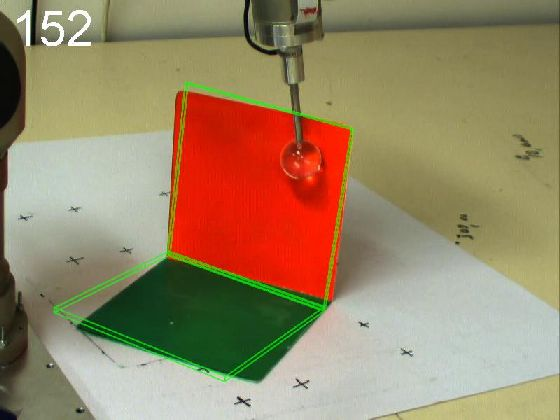
\includegraphics[width=\imgAXwid]{images/A1_2exp_876_2}
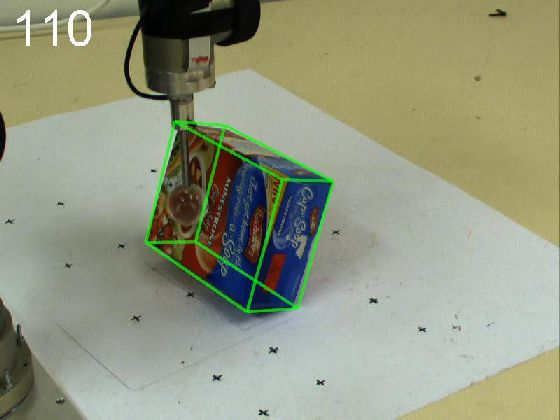
\includegraphics[width=\imgAXwid]{images/A2_2exp_399_2}
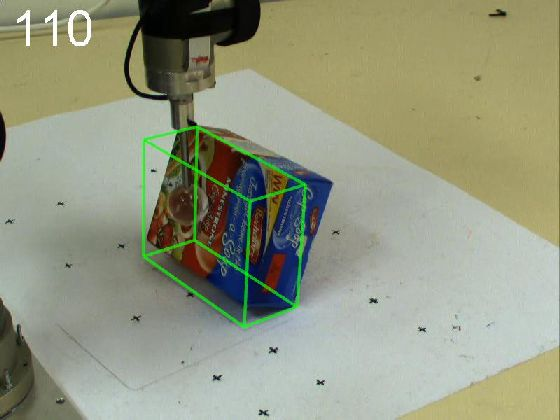
\includegraphics[width=\imgAXwid]{images/A2_LWPR1_399_2}
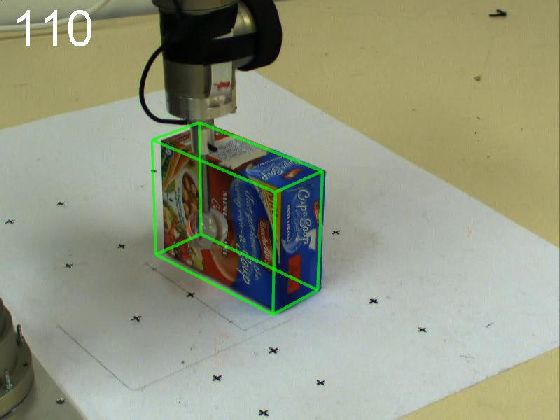
\includegraphics[width=\imgAXwid]{images/A2_2exp_87_2}
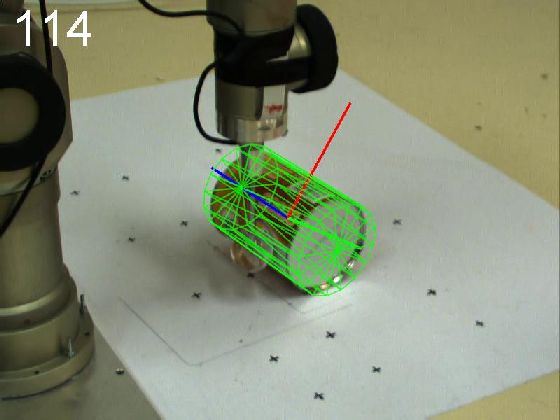
\includegraphics[width=\imgAXwid]{images/A3_2exp_39_2}
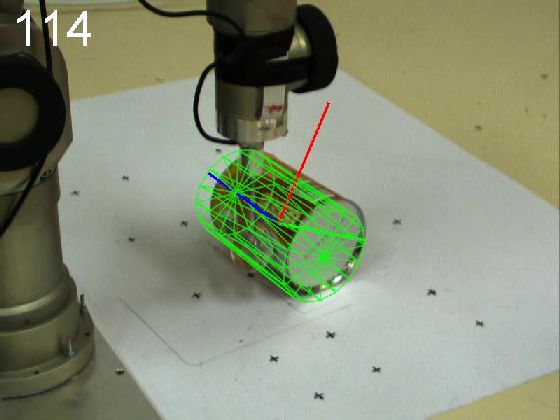
\includegraphics[width=\imgAXwid]{images/A3_LWPR1_39_2}
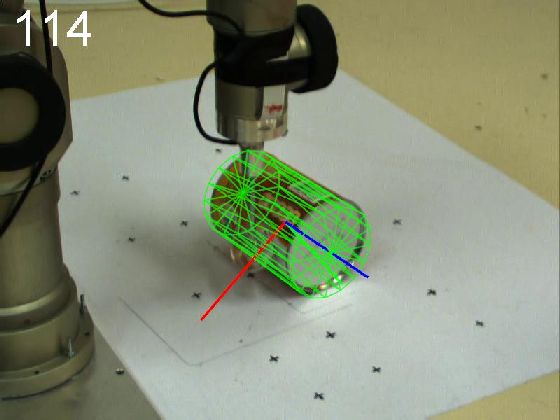
\includegraphics[width=\imgAXwid]{images/A3_physx_39_2}
}
% problem with physx @@@
%\vspace{0.1cm}
%\centerline{
%\includegraphics[width=\imgAXwid]{images/A2_physx_399_1}
%\includegraphics[width=\imgAXwid]{images/A2_physx_399_2}
%\includegraphics[width=\imgAXwid]{images/A2_physx_399_3}
%\includegraphics[width=\imgAXwid]{images/A2_physx_399_4}
%\includegraphics[width=\imgAXwid]{images/A2_physx_399_5}
%}
%\vspace{0.1cm}
\centerline{
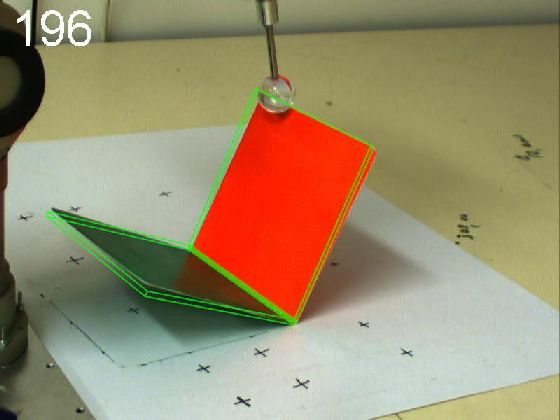
\includegraphics[width=\imgAXwid]{images/A1_2exp_667_3}
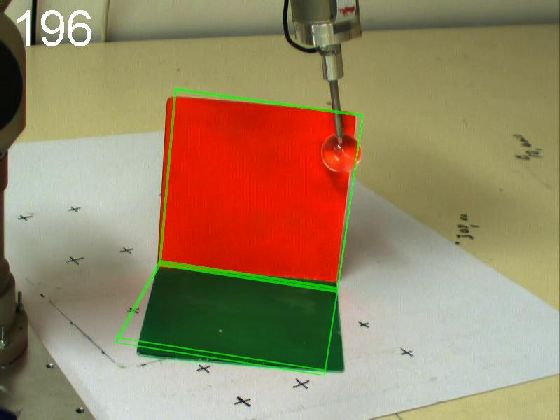
\includegraphics[width=\imgAXwid]{images/A1_2exp_876_3}
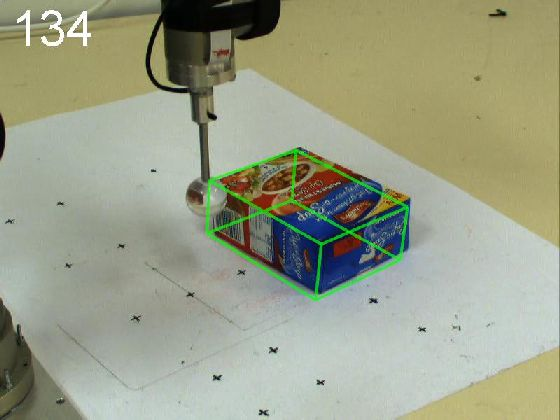
\includegraphics[width=\imgAXwid]{images/A2_2exp_399_3}
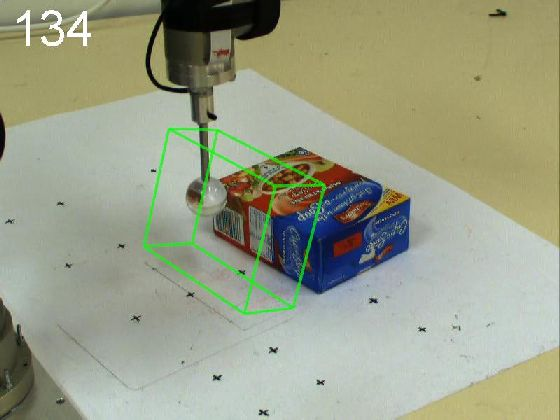
\includegraphics[width=\imgAXwid]{images/A2_LWPR1_399_3}
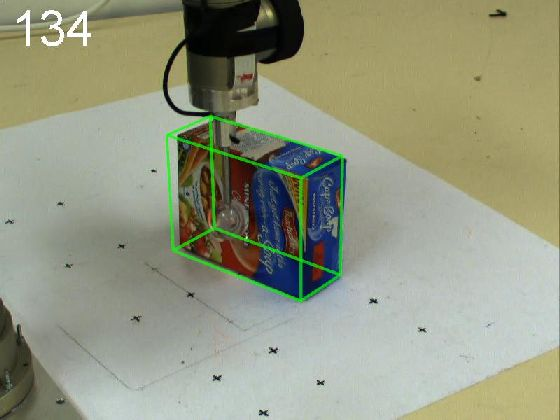
\includegraphics[width=\imgAXwid]{images/A2_2exp_87_3}
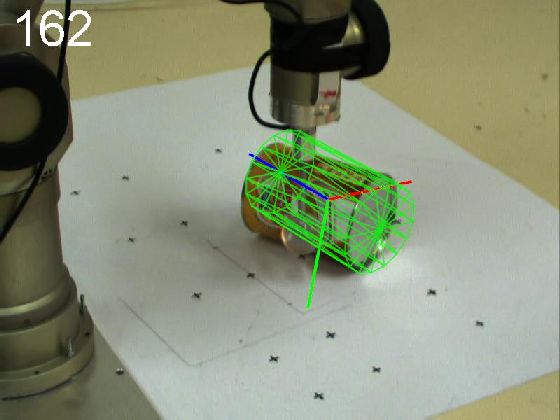
\includegraphics[width=\imgAXwid]{images/A3_2exp_39_3}
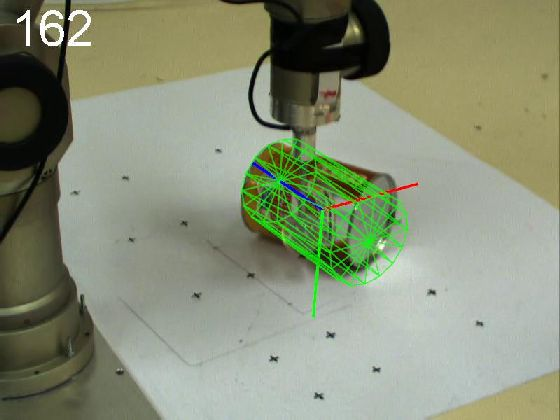
\includegraphics[width=\imgAXwid]{images/A3_LWPR1_39_3}
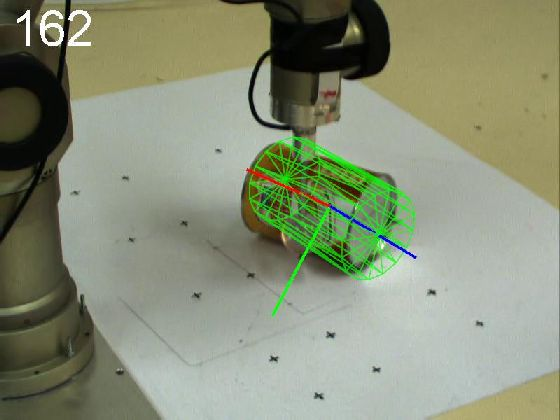
\includegraphics[width=\imgAXwid]{images/A3_physx_39_3}
}
\centerline{
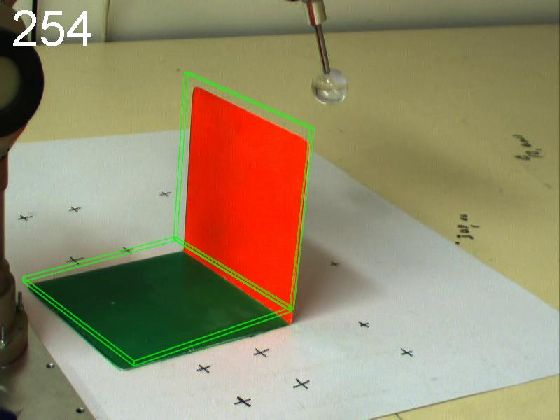
\includegraphics[width=\imgAXwid]{images/A1_2exp_667_4}
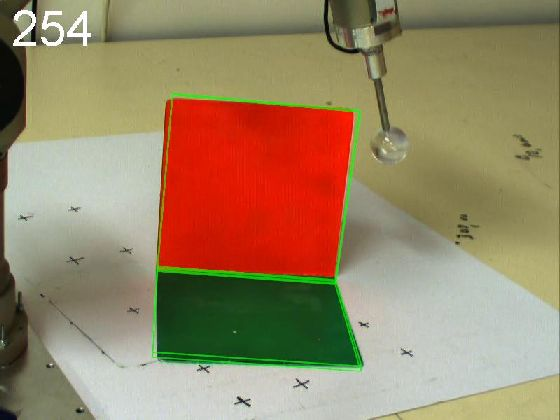
\includegraphics[width=\imgAXwid]{images/A1_2exp_876_4}
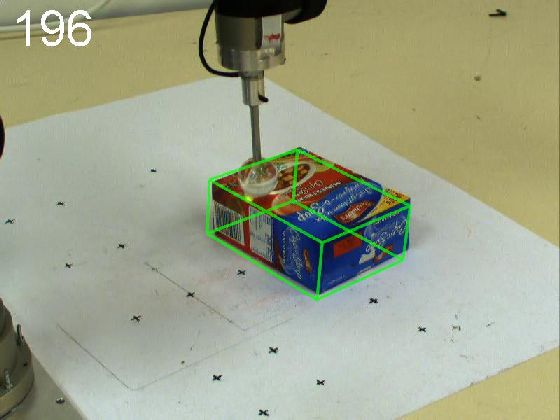
\includegraphics[width=\imgAXwid]{images/A2_2exp_399_4}
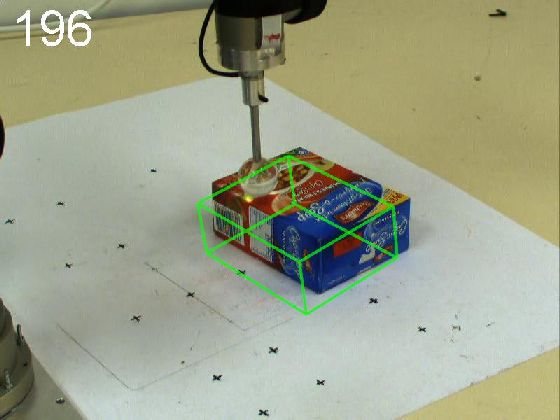
\includegraphics[width=\imgAXwid]{images/A2_LWPR1_399_4}
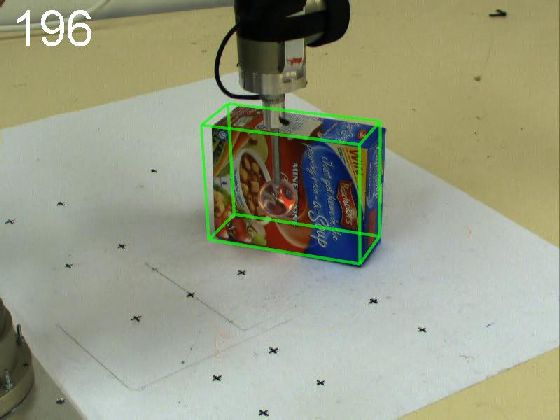
\includegraphics[width=\imgAXwid]{images/A2_2exp_87_4}
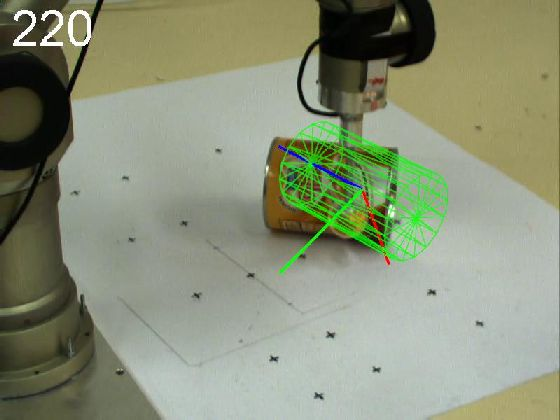
\includegraphics[width=\imgAXwid]{images/A3_2exp_39_4}
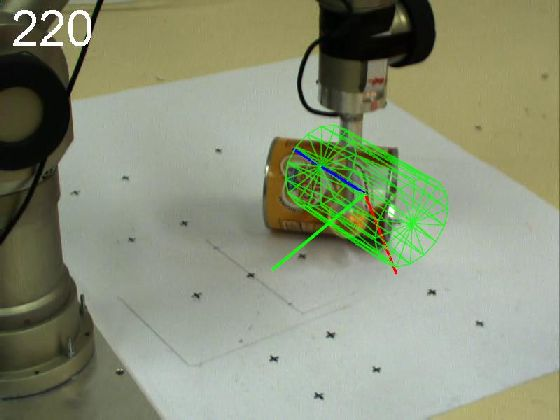
\includegraphics[width=\imgAXwid]{images/A3_LWPR1_39_4}
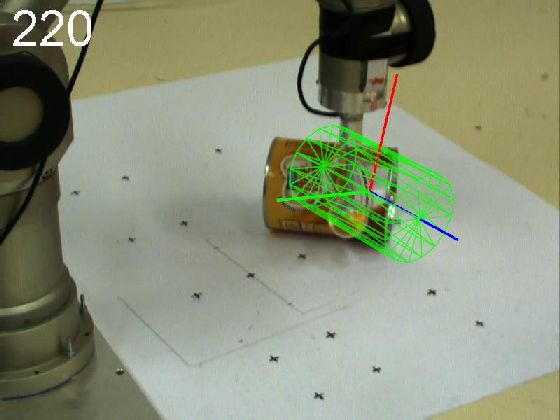
\includegraphics[width=\imgAXwid]{images/A3_physx_39_4}
}
%\vspace{0.1cm}
\centerline{
\includegraphics[width=\imgAXwid]{images/A1_2exp_667_5}
\includegraphics[width=\imgAXwid]{images/A1_2exp_876_5}
\includegraphics[width=\imgAXwid]{images/A2_2exp_399_5}
\includegraphics[width=\imgAXwid]{images/A2_LWPR1_399_5}
\includegraphics[width=\imgAXwid]{images/A2_2exp_87_5}
\includegraphics[width=\imgAXwid]{images/A3_2exp_39_5}
\includegraphics[width=\imgAXwid]{images/A3_LWPR1_39_5}
\includegraphics[width=\imgAXwid]{images/A3_physx_39_5}
}
%\vspace{0.1cm}
\caption {Experiment P1: polyflap, box and cylinder. Green outline shows
  predictions. Columns 1-2: KDEF-GA/quat on two trials exhibiting
  different motions of the polyflap. Col 3: KDEF-GA/quat. Col 4: LWPR-G for one trial in
  which the box topples over. Col 5: KDEF-GA/quat on another trial in
  which the box slides. Columns 6-8 show the same push of the
  cylinder. Col 6: KDEF-GA/quat. Col 7: LWPR-G. Col 8: PhysX. Note tha
  for columns 6-7 the orientation of the cylinder is show by the
  rotating frame. Only the learned models predict the rotation
  correctly.(The
  frame number is shown in the top left of each image.)  }
\label{fig:ExperimentL2}
\end{figure*}
\subsubsection{Experiment P1 discussion} Table~\ref{tab:PerformanceTableL1av} and Figure~\ref{fig:Lgraphs} show that the learned models almost always outperformed the physics simulator on the test set, with approximately one third the prediction error. Thus we find strong support for hypothesis H1. Regarding the parameterisation, Gaussian kernels with quaternions were best in 14 of 15 cases  (Table~\ref{tab:PerformanceTableL1av} boldentries). Thus in experiments P2 and P3 this parameterisation was used for the density estimation algorithms.
In Figure~\ref{fig:ExperimentL2} it can be
seen that predictions were accurate and physically plausible for a
variety of learning methods even over 150 steps. Note the physics
simulator predicts incorrect turning of the cylinder when pushed
(Figure~\ref{fig:ExperimentL2} column 8). Finally Figure~\ref{fig:Lgraphs} shows that additional information A or E gives no advantage for any algorithm in this experiment, indeed LWPR gets worse with more dimensions. This is in line with expectation, since no learning transfer is being attempted.

\subsection{Experiment P2: Action Transfer}
\label{sec:Results.Action}

\begin{figure*}[t]
%\centerline{\includegraphics[width=0.9\columnwidth]{graphs_jw/A_real_sim_av_graph}}
%\centerline{\includegraphics[width=0.45\columnwidth]{graphs_jw/A_sim_av_graph.png}%}
%\centerline{
%\includegraphics[width=0.46\columnwidth]{graphs_jw/A_real_av_graph.png}}
\centerline{\includegraphics[width=0.8\textwidth]{graphs_jw/P2-graphs}}
\caption{Experiment P2: Action transfer. Trained on forward push on polyflap, tested on backward push, for simulated (top) and real data (bottom). Comparative performance of predictors vs. information utilised (global/agent/environment),
as measured by normalised average error ${E_{av}^{norm}}$.
%Also included is a single data point for the PhysX physics engine.
}\label{fig:A_av_graphs}
\end{figure*}

Experiment P2 tests hypothesis H2: whether predictions can be
transfered to novel actions.  The training set was 900 pushes applied to an L shaped flap in one direction (Figure~\ref{fig:ToyExample} top
left).  The test set was 100 pushes applied from the other side (Figure~\ref{fig:ToyExample} top right). The same method was followed in simulation and with the real object. All the algorithm-information variants in Table~\ref{tab:algs} were tested. We measured the transfer prediction error, i.e.\ the prediction error for the novel test actions. Figure~\ref{fig:A_av_graphs} %(also see Table~\ref{tab:PerformanceTableAav})
shows the normalised average error $E_{av}^{norm}$ for the simulation experiment (left panel) and with real objects (right panel).
Figure~\ref{fig:ExperimentA} shows example predicted trajectories on
synthetic and real test cases.

% @@@ COMMENT ON KDE-GAX RESULTS
% \begin{figure*}[tbp]
% \centerline{
% \includegraphics[width=2.3cm]{images/B1_1exp_20_1}
% \includegraphics[width=2.3cm]{images/B1_1exp_20_2}
% \includegraphics[width=2.3cm]{images/B1_1exp_20_3}
% \includegraphics[width=2.3cm]{images/B1_1exp_20_4}
% \includegraphics[width=2.3cm]{images/B1_1exp_20_5}
% }
% \vspace{0.1cm}
% \centerline{
% \includegraphics[width=2.3cm]{images/B1_2exp_20_1}
% \includegraphics[width=2.3cm]{images/B1_2exp_20_2}
% \includegraphics[width=2.3cm]{images/B1_2exp_20_3}
% \includegraphics[width=2.3cm]{images/B1_2exp_20_4}
% \includegraphics[width=2.3cm]{images/B1_2exp_20_5}
% }
% \vspace{0.1cm}
% \centerline{
% \includegraphics[width=2.3cm]{images/B1_3exp_20_1}
% \includegraphics[width=2.3cm]{images/B1_3exp_20_2}
% \includegraphics[width=2.3cm]{images/B1_3exp_20_3}
% \includegraphics[width=2.3cm]{images/B1_3exp_20_4}
% \includegraphics[width=2.3cm]{images/B1_3exp_20_5}
% }
% %\vspace{0.1cm}
% %\centerline{
% %\includegraphics[width=2.3cm]{images/B1_3exp_61_1}
% %\includegraphics[width=2.3cm]{images/B1_3exp_61_2}
% %\includegraphics[width=2.3cm]{images/B1_3exp_61_3}
% %\includegraphics[width=2.3cm]{images/B1_3exp_61_4}
% %\includegraphics[width=2.3cm]{images/B1_3exp_61_5}
% %}
% \caption
% {Experiment A (simulation):
% Green outline shows predictions (from top row to bottom row) by

% compared to simulated `ground truth' (in cyan).
% These predictions illustrate the rationale for extra contact information
% presented in Figure~\ref{fig:ToyExample}.
% (The frame number is shown in the top left of each image.)
% }
% \label{fig:ExperimentA}
% \end{figure*}

\newlength{\imgBXwid}
\setlength{\imgBXwid}{2.07cm}
\begin{figure*}[tb]
\centerline{
\includegraphics[width=\imgBXwid]{images/B1_1exp_20_1}
\includegraphics[width=\imgBXwid]{images/B1_2exp_20_1}
\includegraphics[width=\imgBXwid]{images/B1_3exp_20_1}
\includegraphics[width=\imgBXwid]{images/B2_2exp_58_1}
\includegraphics[width=\imgBXwid]{images/B2_1exp_58_1}
\includegraphics[width=\imgBXwid]{images/B2_LWPR1_58_1}
\includegraphics[width=\imgBXwid]{images/B2_2exp_38_1}
}
%\vspace{0.1cm}
\centerline{
\includegraphics[width=\imgBXwid]{images/B1_1exp_20_2}
\includegraphics[width=\imgBXwid]{images/B1_2exp_20_2}
\includegraphics[width=\imgBXwid]{images/B1_3exp_20_2}
\includegraphics[width=\imgBXwid]{images/B2_2exp_58_2}
\includegraphics[width=\imgBXwid]{images/B2_1exp_58_2}
\includegraphics[width=\imgBXwid]{images/B2_LWPR1_58_2}
\includegraphics[width=\imgBXwid]{images/B2_2exp_38_2}
}
%\vspace{0.1cm}
\centerline{
\includegraphics[width=\imgBXwid]{images/B1_1exp_20_3}
\includegraphics[width=\imgBXwid]{images/B1_2exp_20_3}
\includegraphics[width=\imgBXwid]{images/B1_3exp_20_3}
\includegraphics[width=\imgBXwid]{images/B2_2exp_58_3}
\includegraphics[width=\imgBXwid]{images/B2_1exp_58_3}
\includegraphics[width=\imgBXwid]{images/B2_LWPR1_58_3}
\includegraphics[width=\imgBXwid]{images/B2_2exp_38_3}
}

\centerline{
\includegraphics[width=\imgBXwid]{images/B1_1exp_20_4}
\includegraphics[width=\imgBXwid]{images/B1_2exp_20_4}
\includegraphics[width=\imgBXwid]{images/B1_3exp_20_4}
\includegraphics[width=\imgBXwid]{images/B2_2exp_58_4}
\includegraphics[width=\imgBXwid]{images/B2_1exp_58_4}
\includegraphics[width=\imgBXwid]{images/B2_LWPR1_58_4}
\includegraphics[width=\imgBXwid]{images/B2_2exp_38_4}
}
%\vspace{0.1cm}
\centerline{
\includegraphics[width=\imgBXwid]{images/B1_1exp_20_5}
\includegraphics[width=\imgBXwid]{images/B1_2exp_20_5}
\includegraphics[width=\imgBXwid]{images/B1_3exp_20_5}
\includegraphics[width=\imgBXwid]{images/B2_2exp_58_5}
\includegraphics[width=\imgBXwid]{images/B2_1exp_58_5}
\includegraphics[width=\imgBXwid]{images/B2_LWPR1_58_5}
\includegraphics[width=\imgBXwid]{images/B2_2exp_38_5}
}
\caption
{Experiment P2: Green outline shows predictions. Column 1: KDEF-G/quat. Col 2:
KDEF-GA/quat. Col 3: KDEF-GAE/quat. Col 4: KDEF-GA/quat. Col 5:
KDEF-G/quat. Col 6: LWPR-G. Col 7: KDEF-GA/quat.
Note that the KDEF-G/quat and LWPR-G methods predict
that the robot finger passes through the polyflap.
(The frame number is shown in the top left of each image.)
}
\label{fig:ExperimentA}
\end{figure*}

\subsubsection{Experiment P2 discussion} 
Figure~\ref{fig:A_av_graphs} (left panel) shows that in simulation that additional contact information (A or AE) didn't improve performance of KDE and LWPR. In contrast factorisation could take advantage of the additional information: the performance of KDEF improved significantly. The predictions of KDEF (Figure~\ref{fig:ExperimentA}) precisely match the hypothesised
effects of adding contact information depicted in Figure~\ref{fig:ToyExample} (bottom row). With only global information the finger was predicted by KDEF to pass through the object (Figure~\ref{fig:ExperimentA} column 1). By adding the agent-object information the prediction of KDEF was that the object would move with the finger, but that it penetrated the table (Figure~\ref{fig:ExperimentA} column 2). By also adding object-environment information KDEF predicts that the object will slide along the table in contact with the finger (Figure~\ref{fig:ExperimentA} column 3). On real objects (Figure~\ref{fig:A_av_graphs} right panel) the learned predictors slightly outperform the physics engine, and accuracy of the predictions goes down. But additional contact information with factoring still enables KDEF to make physically plausible predictions. Figure~\ref{fig:ExperimentA} (columns 5 and 6) shows that KDEF-G and LWPR-G predict that the finger passes through the object, and that the object doesn't move. In Figure~\ref{fig:ExperimentA} (columns 4 and 7) KDEF-GA correctly predicts the sliding motion of the object. Only factoring enables this, the unfactored methods don't produce plausible predictions. This supports hypothesis H2: factoring enables action transfer. Transfer is best if the training observations are accurate, diminishing with training noise. 

\subsection{Experiment P3:  Shape Transfer}\label{sec:Results.Shape}
\begin{figure*}[t]
\centerline{\includegraphics[width=0.8\textwidth]{graphs_jw/P3-graphs}}
\caption{Experiment P3: Comparative performance of predictors vs. information utilised, as measured by the normalised average error ${E_{av}^{norm}}$. 
}\label{fig:S_av_graphs}
\end{figure*}
\newlength{\imgCXwid}
\setlength{\imgCXwid}{2.07cm}

\begin{figure*}[t]
%\centerline{
%\includegraphics[width=2.3cm]{images/C1_2exp_48_1}
%\includegraphics[width=2.3cm]{images/C1_2exp_48_2}
%\includegraphics[width=2.3cm]{images/C1_2exp_48_3}
%\includegraphics[width=2.3cm]{images/C1_2exp_48_4}
%\includegraphics[width=2.3cm]{images/C1_2exp_48_5}
%}
%\vspace{0.1cm}
\centerline{
\includegraphics[width=\imgCXwid]{images/C1_2exp_87_1}
\includegraphics[width=\imgCXwid]{images/C1_1exp_87_1}
\includegraphics[width=\imgCXwid]{images/C1_LWPR1_87_1}
\includegraphics[width=\imgCXwid]{images/C5_1exp_6_1}
\includegraphics[width=\imgCXwid]{images/C5_2exp_6_1}
\includegraphics[width=\imgCXwid]{images/C5_3exp_6_1}
\includegraphics[width=\imgCXwid]{images/C2_3exp_75_1}
}
%\vspace{0.1cm}
\centerline{
\includegraphics[width=\imgCXwid]{images/C1_2exp_87_2}
\includegraphics[width=\imgCXwid]{images/C1_1exp_87_2}
\includegraphics[width=\imgCXwid]{images/C1_LWPR1_87_2}
\includegraphics[width=\imgCXwid]{images/C5_1exp_6_2}
\includegraphics[width=\imgCXwid]{images/C5_2exp_6_2}
\includegraphics[width=\imgCXwid]{images/C5_3exp_6_2}
\includegraphics[width=\imgCXwid]{images/C2_3exp_75_2}
}
%\vspace{0.1cm}
\centerline{
\includegraphics[width=\imgCXwid]{images/C1_2exp_87_3}
\includegraphics[width=\imgCXwid]{images/C1_1exp_87_3}
\includegraphics[width=\imgCXwid]{images/C1_LWPR1_87_3}
\includegraphics[width=\imgCXwid]{images/C5_1exp_6_3}
\includegraphics[width=\imgCXwid]{images/C5_2exp_6_3}
\includegraphics[width=\imgCXwid]{images/C5_3exp_6_3}
\includegraphics[width=\imgCXwid]{images/C2_3exp_75_3}
}
\centerline{
\includegraphics[width=\imgCXwid]{images/C1_2exp_87_4}
\includegraphics[width=\imgCXwid]{images/C1_1exp_87_4}
\includegraphics[width=\imgCXwid]{images/C1_LWPR1_87_4}
\includegraphics[width=\imgCXwid]{images/C5_1exp_6_4}
\includegraphics[width=\imgCXwid]{images/C5_2exp_6_4}
\includegraphics[width=\imgCXwid]{images/C5_3exp_6_4}
\includegraphics[width=\imgCXwid]{images/C2_3exp_75_4}
}
%\vspace{0.1cm}
\centerline{
\includegraphics[width=\imgCXwid]{images/C1_2exp_87_5}
\includegraphics[width=\imgCXwid]{images/C1_1exp_87_5}
\includegraphics[width=\imgCXwid]{images/C1_LWPR1_87_5}
\includegraphics[width=\imgCXwid]{images/C5_1exp_6_5}
\includegraphics[width=\imgCXwid]{images/C5_2exp_6_5}
\includegraphics[width=\imgCXwid]{images/C5_3exp_6_5}
\includegraphics[width=\imgCXwid]{images/C2_3exp_75_5}
}

\caption {Experiment P3: Shape Transfer. Green outline shows predictions. Column~1: KDEF-GA/quat.
  Col~2: KDEF-G/quat. Col~3: LWPR-G for one trial.  Note that the
  KDEF-G/quat and LWPR-G methods predict that the robot finger moves
  into the box.  Col~4: KDEF-G/quat. Col~5: KDEF-GA/quat. Col~6:
  KDEF-GAE/quat. Col~7: KDEF-GAE/quat. The frame number is shown in
  the top left of each image.  }
\label{fig:ExperimentStransfer}
\end{figure*}


Experiment P3 tests hypothesis H3: can predictors learned from one or two objects transfer their predictions to an object of novel shape? The experiment was run in simulation and with real objects. Shape transfer was tested from i) a polyflap to a box (P3.A) and ii) a box and a cylinder to a double cylinder (P3.B). There were 900 training pushes on the polyflap and 200 test pushes on the box for i), and 200 training pushes (100 box, 100 cylinder) and 100 test pushes (double cylinder) for ii). This experiment ran on real objects for i) and ii) and in simulation for i), giving three train-test conditions in total. We have previously published results from simulation for i) \citep{kopicki-etal-icra11}. All algorithm-information combinations from Table~\ref{tab:algs} were tried. When learning from two objects the same number of factors (experts) were used for each object, and they were matched across the two objects by hand. This means each expert received a mix of data from each object, learning to encode both rolling and sliding or tipping motions.  The normalised average error for all three conditions $E_{av}^{norm}$ is shown in Figure~\ref{fig:S_av_graphs}. Example frames from the experiments are shown in Figure~\ref{fig:ExperimentStransfer}.

\subsubsection{Experiment P3 discussion} Shape transfer only occurs with additional contact information and with factoring, such as for the
KDEF-GA method in experiment P3.A (Figure~\ref{fig:ExperimentStransfer} column 1).  Learners with global information only predict that the finger passed  through the box (Figure~\ref{fig:ExperimentStransfer} columns 2 and 3). In experiment P3.A, of the learners, only factoring plus all the contact information (KDEF-GAE) produced physically plausible predictions. In Figure~\ref{fig:ExperimentStransfer} (column 6) KDEF-GAE predicts that the double-cylinder slides along the table, whereas KDEF-G and KDEF-GA predict it will penetrate the table (Figure~\ref{fig:ExperimentStransfer} columns 4 and 5). KDEF-GAE also makes physically plausible predictions for a novel real object 
(Figure~\ref{fig:ExperimentStransfer} column 7). None of the other learners could achieve this shape transfer learning. Only by using factoring plus all contact information was shape transfer learning achieved. In fact KDEF-GAE also matched the accuracy of the physics simulator. Thus this experiment supports hypothesis H3: factoring + contact information enables shape transfer learning.

\subsection{General Discussion} 

There are two questions that arise from the experiments collectively. First why does PhysX fail to do better P1 even though separately tuned to each object? The answer is that real objects don't adhere to idealised friction models with one coefficient for each surface: flaws in object surfaces cause deviations from the tuned model. Thus the problem holds for all such simulators and so a modular learning model will always be better. Second, why does transfer learning decline on real data in P2 and P3? The answer is tracking noise in the training data, leading to perceived penetrations of the object by the finger, giving some probability in the model that the finger can pass through the object. 
%***ADD IMAGES TO ILLUSTRATE HOW LWPR ALWAYS REMAINS STATIONARY WHILE KDE PREDICTS MOTIONS!!!***

% @@@ COMMENT ON KDE-GAX RESULTS



%%%%%%%%%%%%%%%%%%%%%%%%%%%%%%%%%%%%%%%%%%%%%%%%%%%%%%%%%%%%%%%%%%%%%%%
%% Experiment S2

%\subsubsection{Training on a box and a cylinder, and testing on two rigidly connected cylinders}


% @@@ COMMENT ON KDE-GAX RESULTS

% PROBLEM THAT C5 TRAINED ON ONLY 100 box + 100 cyl
% whereas C2 trained on 500 box + 100 cyl


%\begin{figure}[htbp]
%\centerline{\includegraphics[width=\the\barchartwidth]{S2_sim_av_graph}}
%\centerline{\includegraphics[width=\the\barchartwidth]{S2_real_av_graph}}
%\caption{Experiment S2: Generalisation to novel shape.
%Trained on cylinder and box, tested on double-cylinder,
%for simulated (top) and real data (bottom).%
%Comparative performance of predictors vs. information utilised,
%as measured by the normalised average error ${E_{av}^{norm}}$.}
%\label{fig:S2_av_graphs}
%\end{figure}


% @@@ COMMENT ON KDE-GAX RESULTS, WHICH ARE THE BEST !!!

%\begin{figure}[htbp]
%\centerline{\includegraphics[width=\the\barchartwidth]{graphs_jw/S3_sim_av_graph.png}}
%\caption{Experiment S3: Interpolative generalisation to novel shape.
%Trained with downward pushes on angled polyflaps,
%tested on similar polyflaps, using simulated data.
%Comparative performance of predictors vs. information utilised,
%as measured by the normalised average error ${E_{av}^{norm}}$.}
%\label{fig:S3_av_graph}
%\end{figure}


% \begin{figure*}[htbp]
% \centerline{
% \includegraphics[width=2.3cm]{images/C5_1exp_6_1}
% \includegraphics[width=2.3cm]{images/C5_1exp_6_2}
% \includegraphics[width=2.3cm]{images/C5_1exp_6_3}
% \includegraphics[width=2.3cm]{images/C5_1exp_6_4}
% \includegraphics[width=2.3cm]{images/C5_1exp_6_5}
% }
% \vspace{0.1cm}
% \centerline{
% \includegraphics[width=2.3cm]{images/C5_2exp_6_1}
% \includegraphics[width=2.3cm]{images/C5_2exp_6_2}
% \includegraphics[width=2.3cm]{images/C5_2exp_6_3}
% \includegraphics[width=2.3cm]{images/C5_2exp_6_4}
% \includegraphics[width=2.3cm]{images/C5_2exp_6_5}
% }
% \vspace{0.1cm}
% \centerline{
% \includegraphics[width=2.3cm]{images/C5_3exp_6_1}
% \includegraphics[width=2.3cm]{images/C5_3exp_6_2}
% \includegraphics[width=2.3cm]{images/C5_3exp_6_3}
% \includegraphics[width=2.3cm]{images/C5_3exp_6_4}
% \includegraphics[width=2.3cm]{images/C5_3exp_6_5}
% }
% %\vspace{0.1cm}
% %\centerline{
% %\includegraphics[width=2.3cm]{images/C5_3exp_12_1}
% %\includegraphics[width=2.3cm]{images/C5_3exp_12_2}
% %\includegraphics[width=2.3cm]{images/C5_3exp_12_3}
% %\includegraphics[width=2.3cm]{images/C5_3exp_12_4}
% %\includegraphics[width=2.3cm]{images/C5_3exp_12_5}
% %}
% \caption {Experiment S-transfer: extrapolative generalisation to novel
%   shape (simulation): Green outline shows predictions (from top row to
%   bottom row) by KDEF-G/quat, KDEF-GA/quat, and KDEF-GAE/quat,
%   compared to simulated `ground truth' (in cyan).  Note that the -G
%   and -GA methods predict that the object moves into and through the
%   ground plane.  (The frame number is shown in the top left of each
%   image.)  }
% %\todo[color=\MK,inline]{MK: generate side pushes for S2sim (=C5)}
% \label{fig:ExperimentStransfer}
% \end{figure*}


% \begin{figure*}[htbp]
% %\centerline{
% %\includegraphics[width=2.3cm]{images/C2_3exp_27_1}
% %\includegraphics[width=2.3cm]{images/C2_3exp_27_2}
% %\includegraphics[width=2.3cm]{images/C2_3exp_27_3}
% %\includegraphics[width=2.3cm]{images/C2_3exp_27_4}
% %\includegraphics[width=2.3cm]{images/C2_3exp_27_5}
% %}
% %\vspace{0.1cm}
% \centerline{
% \includegraphics[width=2.3cm]{images/C2_3exp_75_1}
% \includegraphics[width=2.3cm]{images/C2_3exp_75_2}
% \includegraphics[width=2.3cm]{images/C2_3exp_75_3}
% \includegraphics[width=2.3cm]{images/C2_3exp_75_4}
% \includegraphics[width=2.3cm]{images/C2_3exp_75_5}
% }
% \caption {Experiment S-transfer: extrapolative generalisation to novel
%   shape (real data): Green outline shows prediction by KDEF-GAE/quat.
%   (The frame number is shown in the top left of each image.)  }
% \label{fig:ExperimentStransfer}
% \end{figure*}







%\clearpage

%%%%%%%%%%%%%%%%%%%%%%%%%%%%%%%%%%%%%%%%%%%%%%%%%%%%%%%%%%%%%%%%%%%%%%%
%
%${E_{av}^{norm}} \pm se$
%C4.polyflap.1explf & 0.097 $\pm$ 0.002 \\

%${E_{f}^{norm}} \pm se$
%C4.polyflap.1explf & 0.257 $\pm$ 0.006 \\

